\section{Results} 
We consider an animal who interacts with an environment over a sequence of states, actions and rewards, embedded in the now standard Markov decision process. The goal is to select actions in a way that maximizes the total reward collected from the environment. 

% TODO - notation....

If the animal has incomplete knowledge of the environment challenge it faces in this kind learning to maximize reward is to succeed in the tradeoff between exploration and exploitation. The standard way of approaching this problem is well described by \cite{Sutton2018} who wrote,

\begin{quotation}
	The agent must try a variety of actions and progressively favor those that appear to be best. 	
\end{quotation}

Here we suggest two fairly radical changes. Don’t stop searching progressively, do so suddenly. Explore only out of curiosity. 

Why curiosity? Curiosity is a rational behavoir \cite{Rich2016a}, or so we argue. Curiousity is just as important for survival as reward collection \cite{Thrun1992}. Curiosity is a primary drive in most, if not all, animals \cite{Inglis2001}. It is as strong, if not sometimes stronger, than the drive for reward \cite{Loewenstein1994,Kidd2015,Gottlieb2018}. Curiosity, as an algorithm, is highly effective at solving optimization problems \cite{Schmidhuber1991,Pathak2017,Stanton2018,Lehman201,Mouret2011b1,Fister2019,Mouret2015,Colas2020,Cully2015,Pathak2017,Schwartenbeck2019.Laversanne-Finot2018}. In short, curiosity is necesssary, omnipresent, and effective.

But what is curiosity? Curiosity is an open-ended search to learn any information, informally speaking \citep{Kidd2015}. Working models of curiosity tend to conflate the learning rule, with the objective itself. We will now describe an optimal value, but deterministic model, of curiosity. It is defined by some easily satisfiable requirements (axioms). This basis makes curiosity domain general, and learning rule independent. We do assume it should be value driven, and as time-efficient as possible.


\subsection{Memory and learning} 
% TODO - cites
Sustained firing, the strength between two synapses, elevated Calcium concentration are three simple examples of learning and memory in the nervous system. A chalk board after a lecture and a picture of this written page are two examples of embodied memory. An hard drive, or old fashion punch cards, are two examples of computer memory. Each of these can though be represented as a vector space. Generally we will regard memory $\Theta$ as encoding a sequence of observations X, that have arrived via a communications channel $C$. A learning function can be any function $f$ that maps observations into memory $\Theta$. And function f is considered to be a valid learning function as long as the mapping changes $\Theta$ some small amount. The function $f$ offers a non-constant mapping, in other words.

We would like to describe curiosity in this general way because in ecologically-speaking curiosity does not seem to depend on any one single kind of learning. Curiosity will depend on many different mechanisms of memory and learning. The most general definition of curiosity would allow for any kind of learning. So this is the setting we have chosen. We will now describe this new formalism, and try and prove it is a useful one.

The question we now consider is how to value the information from a channel $C$. If the communication channel who output we are valuing is agnostic to semantics, we assume value should be as well. We argue the value information from a channel can be stated in terms of the dynamics of memory alone, as we will know show. As seems clear, our setting for defining information value closely follows that of Shannon and his definition of a communication channel.

As has been common elsewhere \cite{Schmidhuber1991,Oudeyer2016,Pathak2017,Gottlieb2018,Wilson2020,Schwartenbeck2019} we do not assume that $f$ has only one objective to say minimize the error between the memory and the observation. We instead assume the learning function is chosen to be well suited for survival, loosely defined, in the environment and neural circuits for which it will operate, and for the kinds of observations it may encode. If the memory is a computer memory, and $f$ represents a learning function for simple linear regression then error may in fact be minimized. If error is the memory of a child or a human adult, then it is entirely possible learning will inspire a new idea, insight, imagination, or novely approach. It others, we argue that not every curious action is driven to itself minimize uncertainty.

Formally, any notion of information value requires that there must be a memory, $\Theta$, and a way to learn, $f$. For our general mathematical theory we will define memory as,

\begin{itemize}
\item A set of real valued numbers
\item Embedded in a finite space, with $N$ dimensions 
\item Closed and bounded
\end{itemize}

We define learning in a matching way. A learning function \textit{can be any function} that maps observations $x$ into memory. Using the function-arrow notation this kind of learning is denoted by, $f(x;\Theta) \rightarrow \Theta'$. Likewise a forgetting function \textit{can be any function} that inverts the memory, $f^{-1}(x;\ \Theta') \rightarrow \Theta$. 

So what are observations? It is convenient to assume that all observations are also embedded in a finite real space, $x \sim X \in \mathbb{R}^m$, as are actions $a \sim A \in \mathbb{R}^k$, and that rewards are positive real numbers, $R \in \mathbb(R^{+})$. 

In calling them ``observations'' we do not mean to imply they must arise from the senses, or direct from states $S$. Observations could be internally generated from thought, or externally generated from the senses or from the environment, Or both in combination, as is common to recurrent neural networks . Observations may contain action information, or they may not. Observations may contain reward information, or they may not. Our account of learning has no preference.

\subsection{Information value} 
Treating memory as vector space, and our open-ended definition of learning, are two of the essential and innovative ideas we use to define information value in agnostic terms. The third and final piece, again taking the lead from Shannon, it to rest our final result on some easily satisfied requirements (axioms).

So we have a memory $\Theta$, which has been learned by $f$ over a history of observations, $[f(x_0; \Theta_0), f(x_1; \Theta_1), f(x_2; \Theta_2), \ldots]$. Can we measure how much value the next observation $f(x_t)$ should have? We think this measure $E$ should have certain properties.

\begin{enumerate}
	\item $E$ should depend only on a memory, and what can be immediately learned. ($x$, $\Theta$, and $f$)
	\item An observation that is known completely, or cannot be learned, should have a value of 0. (If $\Delta \Theta = 0$, then $E=0$)
	\item $E$ should be non-negative because learning is never itself harmful. ($E \ge 0$)
	\item $E$ should increase monotonically with the change in memory. ($E \propto \Delta \Theta$)
	\item $E$ for the same observation should become decelerating in finite time. ($E \rightarrow 0$ as $t \rightarrow T^*$)
\end{enumerate}

These properties are in part inspired by Shannon's axioms for information theory, and in part borrowed from other's theories of information maximization \cite{Itti2009,Jaegle2019,Schmidhuber1991}, and information foraging \citep{Inglis2001,Reddy2016,Pirolli2007}. What we have done is remove Bayes rule, or any explicit learning rule, and replaced some general requirments (our axioms). This is important not for its own sake, but because anything we prove in this  setting must be true for any learning algorithm. This includes Bayesian reasoning. 

We can satisfy all these properties by taking a geometric view of learning using two definitions. They are also shown graphically in Fig.~\ref{fig:cartoon} and described in detail in Boxes ~\ref{box:norm}-\ref{box:laplacian}.

\begin{itemize}
	\item[] \textbf{Definition 1} Let $E$ be the norm of $|| f_{\Theta}(x) - \Theta ||$.	
	\item[] \textbf{Definition 2} Let $|| f_{\Theta}(x)||$ be constrained such that $\nabla^2 \Theta < 0$ for all $ t \ge T^*$. 	
\end{itemize}

\begin{figure}
	\begin{fullwidth}
	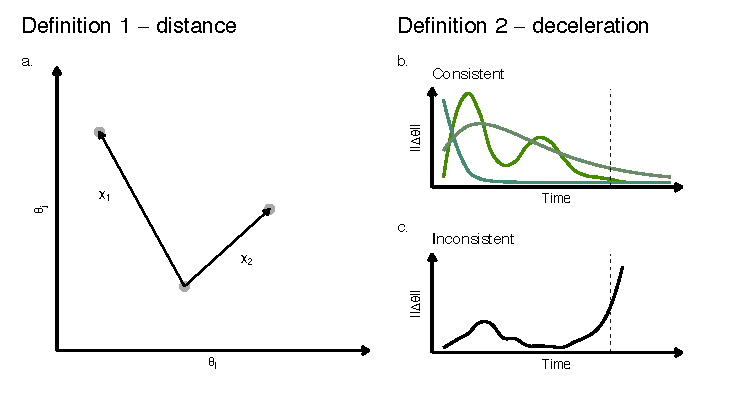
\includegraphics[width=0.7\linewidth]{img/cartoon.pdf} 
	\caption{A diagram of our definitions. 
	\textbf{a}. This panel illustrates a two dimensional memory. The information value of two observations $x_1$ and $x_2$ depends on the norm of memory with learning. Here we show this distance as a euclidean norm, denoted as a black arrow.
	\textbf{b-c} This panel illustrates learning dynamics with time (over a series of observations that are not shown). If information value becomes decelerating in finite time bound, then we say that learning is consistent with Def. 2. This is shown in panel b. The bound is depicted as a dotted line. If learning does not decelerate, then it is said to be inconsistent with Def. 2 (Panel c). \textit{It is important to note:} our account of curiosity does not apply when learning is inconsistent.
  	}
	\label{fig:cartoon} 
	% \figsupp{} % No limit on these.
	\end{fullwidth}
\end{figure}

% --------------------------------------------------------------------------
\begin{featurebox}
\caption{Norms.}
\label{box:norm}
A \textbf{norm} is a mathematical way to measure the overall size or extent of an ``object'' in a space. The object we are concerned with is a mathematical object with a form given by, $\Delta \Theta = f_{\Theta}(x) - \Theta$. But to define the norm let us as the first step consider a generic vector $v$. Keeping with convention will have its norm denoted by $||v||$, and defined by three properties:

\begin{enumerate}
  \item $||v|| > 0$ when $v \neq 0$ and $||v|| = 0$ only if $v=0$ (point separating)
  \item $||k v|| = ||k||\ ||v||$ (absolute scalability)
  \item $||v + w|| \leq ||v|| + ||w||$ (the triangle inequality)
\end{enumerate}

What does this mean for $\Delta \Theta$? A norm over a changing memory provides most the properties we require for our definition of $E$. It depends only on learning (and forgetting), that dependence must be monotonic, a norm is zero only when nothing in the space/memory changes and is positive definite. These satisfy the first four properties. For the fifth, see Box \ref{box:laplacian}.
\medskip
\end{featurebox}

\begin{featurebox}
	\caption{The Laplacian.}
	\label{box:laplacian}
	Here we use $\nabla^2$ to represent the \textbf{Laplacian}, which provides the second derivative of vector valued functions, giving us the remaining property we need. (See Box \ref{box:norm} for the others). To explain why, suppose we are working with a 1- dimensional memory. In this case the Laplacian reduces to the second derivative on our memory, $\frac{d^2\Theta}{dx^2} < 0$. A negative second derivative will force the changes in memory to be decelerating, by definition. In higher dimensions of memory then, a reader can think of the Laplacian as the ``second derivative'' of vector-valued functions like $f$. That is, negative Laplacian imply decelerating by definition.
	\medskip
\end{featurebox}
% --------------------------------------------------------------------------

% TODO clean this; need to end with concrete examples?
% We choose these definitions because their minimalism makes them extremely general, covering all modes of working or episodic memory (17, 18), probabilistic memory (19–21), count-based memory, predictive coding, and even memories based categorization, compression or latent-states (22, 23). 

\subsection{Exploration as a dynamic programming problem}
Curiosity is a search to maximize information value, again in the broadest sense possible. We decided to seek a dynamic programming solution to maximizing curiosity \citep{Bellmann1954}. This is useful because it would guarantee value is maximized, which, because of the way we have made our definitions, also guarantees that learning is complete. It is also convenient because dynamic programming is the basis for reinforcement learning \citep{Sutton2018}. 

The normal route to find a dynamic programming solution is to first prove your problem has ``optimal substructure'', then to derive the final result using Bellman optimality, and this is the route we will follow. For a more complete introduction to optimal substructure, see Box~\ref{box:substructure}. For more on dynamic programming and Bellman optimality, see Box~\ref{box:bellman}. 

In Theorem~\ref{theorem:opt_sub} (mathematical appendix) we prove our definition of memory has optimal substructure. This proof relies on the forgetting function $f^{-1}$ to succeed. Even though we have said little about it until now, this is why we include forgetting in our early definitions. 

% -------------------------------------------------------------------------
\begin{featurebox}
	\caption{Optimal substructure}
	\label{box:substructure}
	To use Bellman's principle of optimality (Box~\ref{box:bellman}) the problem we want to solve needs to have \textbf{optimal substructure}. This opaque term can be understood by looking in turn at another theoretical construct, Markov spaces. 
	\\
	In Markov spaces there are a set of states or observations $(x_0, x_1, ..., x_{T})$, where the transition to the next $x_t$ depends only on the previous state $x_{t-1}$. This limit means that if we were to optimize over these states, as we do in reinforcement learning, we know that we can treat each transition as its own ``subproblem'' and therefore the overall situation has ``optimal substructure''.
	\\
	In reinforcement learning the problem of reward collection is defined by fiat as happening in a Markov space \citep{Sutton2018}. The problem for curiosity is it relies on memory which is necessarily composed of many past observations, in many orders, and so it cannot be a Markov space. So if we wish to use dynamic programming to maximize $E$, we need to find another way to establish optimal substructure. This is the focus of Theorem~\ref{theorem:opt_sub}.
	\medskip
\end{featurebox}
% -------------------------------------------------------------------------

% -------------------------------------------------------------------------
\begin{featurebox}
	\caption{Dynamic programming and Bellman optimality.}
	\label{box:bellman}
	The goal of dynamic programming is to find a series of actions $(a_1, a_2, ..a_T)$, drawn from a set $A$, that maximize each payout $(r_1, r_2, ..., r_{T})$ so the total payout received is as large as possible. If there is a policy $a = \pi(x)$ to take actions, based on a series of observations $(x_0, x_1, ..x_{T}),$, then an optimal policy $\pi^*$ will always find the maximum total value $V^* = \argmax_{A} \sum_T r_t $. The question that Bellman and dynamic programming solve then is how to make the search for finding $\pi*$ tractable. In the form above one would need to reconsider the entire sequence of actions for any one change to that sequence, leading to a combinatorial explosion. 
	
	Bellman's insight was a way to make the problem simpler, and break it down into a small set of problems that we can solve in a tractable way without an explosion in complexity. This is his principle of optimality, which reads:

	\begin{quote}
		An optimal policy has the property that whatever the initial state and initial decision are, the remaining decisions must constitute an optimal policy with regard to the state resulting from the first decision. \citep{Bellmann1954}
	\end{quote}

	Mathematically this allows us to translate the full problem, $V^* = \argmax_{\pi} \sum_T r_1, r_2, ..., r_{T}$ to a recursive one, which is given below. 

	\begin{equation}
		V^* = \argmax_{\pi} \ \Big [ r_0 + V(x_1) \ \Big ]
	\end{equation}
	
	Using this new form we can find an optimal solution by moving though the sequence of action iteratively, and solving each step independently. The question which remains though is how can we ensure our problem can be broken down this way? This is addressed in Box~\ref{box:substructure}.
	\medskip
\end{featurebox}
% -------------------------------------------------------------------------

The Bellman derivation leads to an especially practical and simple result (Eq.~\ref{eq:V_E}). Given an arbitrary starting value $E_0 > 0$, the dynamic programming solution to maximizing $E$ is given by Eq.~\ref{eq:V_E_bellman}. A full derivation is provided in the mathematical appendix. We denote our policy that follows this solution as $\pi_E$.

\begin{equation}
	\label{eq:V_E_bellman} 
	V^{\pi}_E(x) = \argmax_A \Big [ E_0 + V_E(x_1) \Big ]
\end{equation}

However as long learning about the different states $x$ is independent, and as long as learning continues until steady-state, $E_t =0$, then there are many equally good solutions to the search. Under these conditions we can simplify Eq. \ref{eq:V_E_bellman} further, giving Eq. \ref{eq:EE}. 

\begin{equation}
	\label{eq:EE} 
	V^{\pi}_E(x) = \argmax_A \Big [ E_0 + E(x_1) \Big ]
\end{equation}

\subsection{Optimal exploration, and the importance of boredom}
What would it mean for a curiosity search to be efficient? Does our Bellman solution ensure it?

Exploration is limited in practice by available energy, hunger, greed, thirst and other biological priorities. More importantly search should be limited to avoid the central failure of curiosity: it can become distracted by what we call minutia. Those details which have no use. A good example of this was given by \cite{Pathak2017} who asks us to, ``Imagine a scenario where the agent is observing the movement of tree leaves in a breeze. Since it is inherently hard to model breeze, it is even harder to predict the location of each leaf''. This will imply, they note, that a curious agent will always remain curious about the leaves, to its own detriment. 

To limit curiosity we will draw on its opposite, boredom, which we consider to be an adaptive trait. Others have considered boredom this way, arguing it is a useful way to motivate aversive tasks \citep{Bench2013}. We take a slightly different view and consider boredom as a means to ignore the marginal. We treat it as a tunable free parameter, $\eta \ge 0$, and then say all curious exploration should cease once $E \le \eta$. In other words, once learning becomes marginal the action policy must change, as given by Eq.~\ref{eq:null}. 

\begin{equation}
	\label{eq:null}
	E \le \eta : \pi_E \rightarrow \pi_{\emptyset}
\end{equation}

We use $\pi_{\emptyset}$ to denote any other action policy that is not $\pi_E$. Informally Eq.~\ref{eq:null} means that once $E$ is below the boredom threshold, E is marginal, and the learner should change its behavior from exploration to some other policy. This change in behavior could be towards an aversive policy (as in \citep{Bench2013}) or it could be towards reward seeking, as we will assume.

We think it is reasonable to call a curious search optimal if it meets the three criteria below. 

\begin{enumerate}
	\item Exploration should visit all available states of the environment at least once.
	\item Exploration should cease when learning has plateaued.
	\item Exploration should take as few steps as possible to achieve 1 and 2.
\end{enumerate}

In Theorem~\ref{needed} we prove that $\pi_E$ satisfies these, when $\eta > 0$.

\subsection{Information collection}
The work so far has built up the idea that the most valuable, and most efficient, curious search will come from a deterministic algorithm. That is, every step strictly maximizes $E$. It is this determinism which will let us resolve the dilemma, later on. A deterministic view of exploration seems at odds with how the problem is generally viewed today, which involves searching with some amount of randomness. Whereas if our analysis is correct, randomness is not needed or desirable, as it must lead to less value and a longer search. 

We confirm and illustrate this result using an example of a simple information foraging task (Task 1; Fig.\label{fig:task_outline1}). This variation of the bandit task \citep{Sutton2018} replaces rewards with information, in this case colors. On each selection, the agent sees one of two colors according to a specific probability shown in Fig. ~\ref{fig:payout}a. When the relative color probabilities are more similar that arm has more entropy and so more to learn and more information value. Arms that are certain to present only one color lose their informative value quickly.

The results of this simple information seeking task are shown in Figure~\ref{fig:curiosity1}. Deterministic curiosity in this task generated more information value, in less time, and with zero regret when compared against a stochastic agent using more directed random search. As our work here predicts, noise only made the search happen slower and lead to regret. Besides offering a concrete example, performance in Task 1 is a first step in showing that even though $\pi_E$'s optimality is proven for a deterministic environment, it can perform well in other settings.

\begin{figure}
	\begin{fullwidth}
	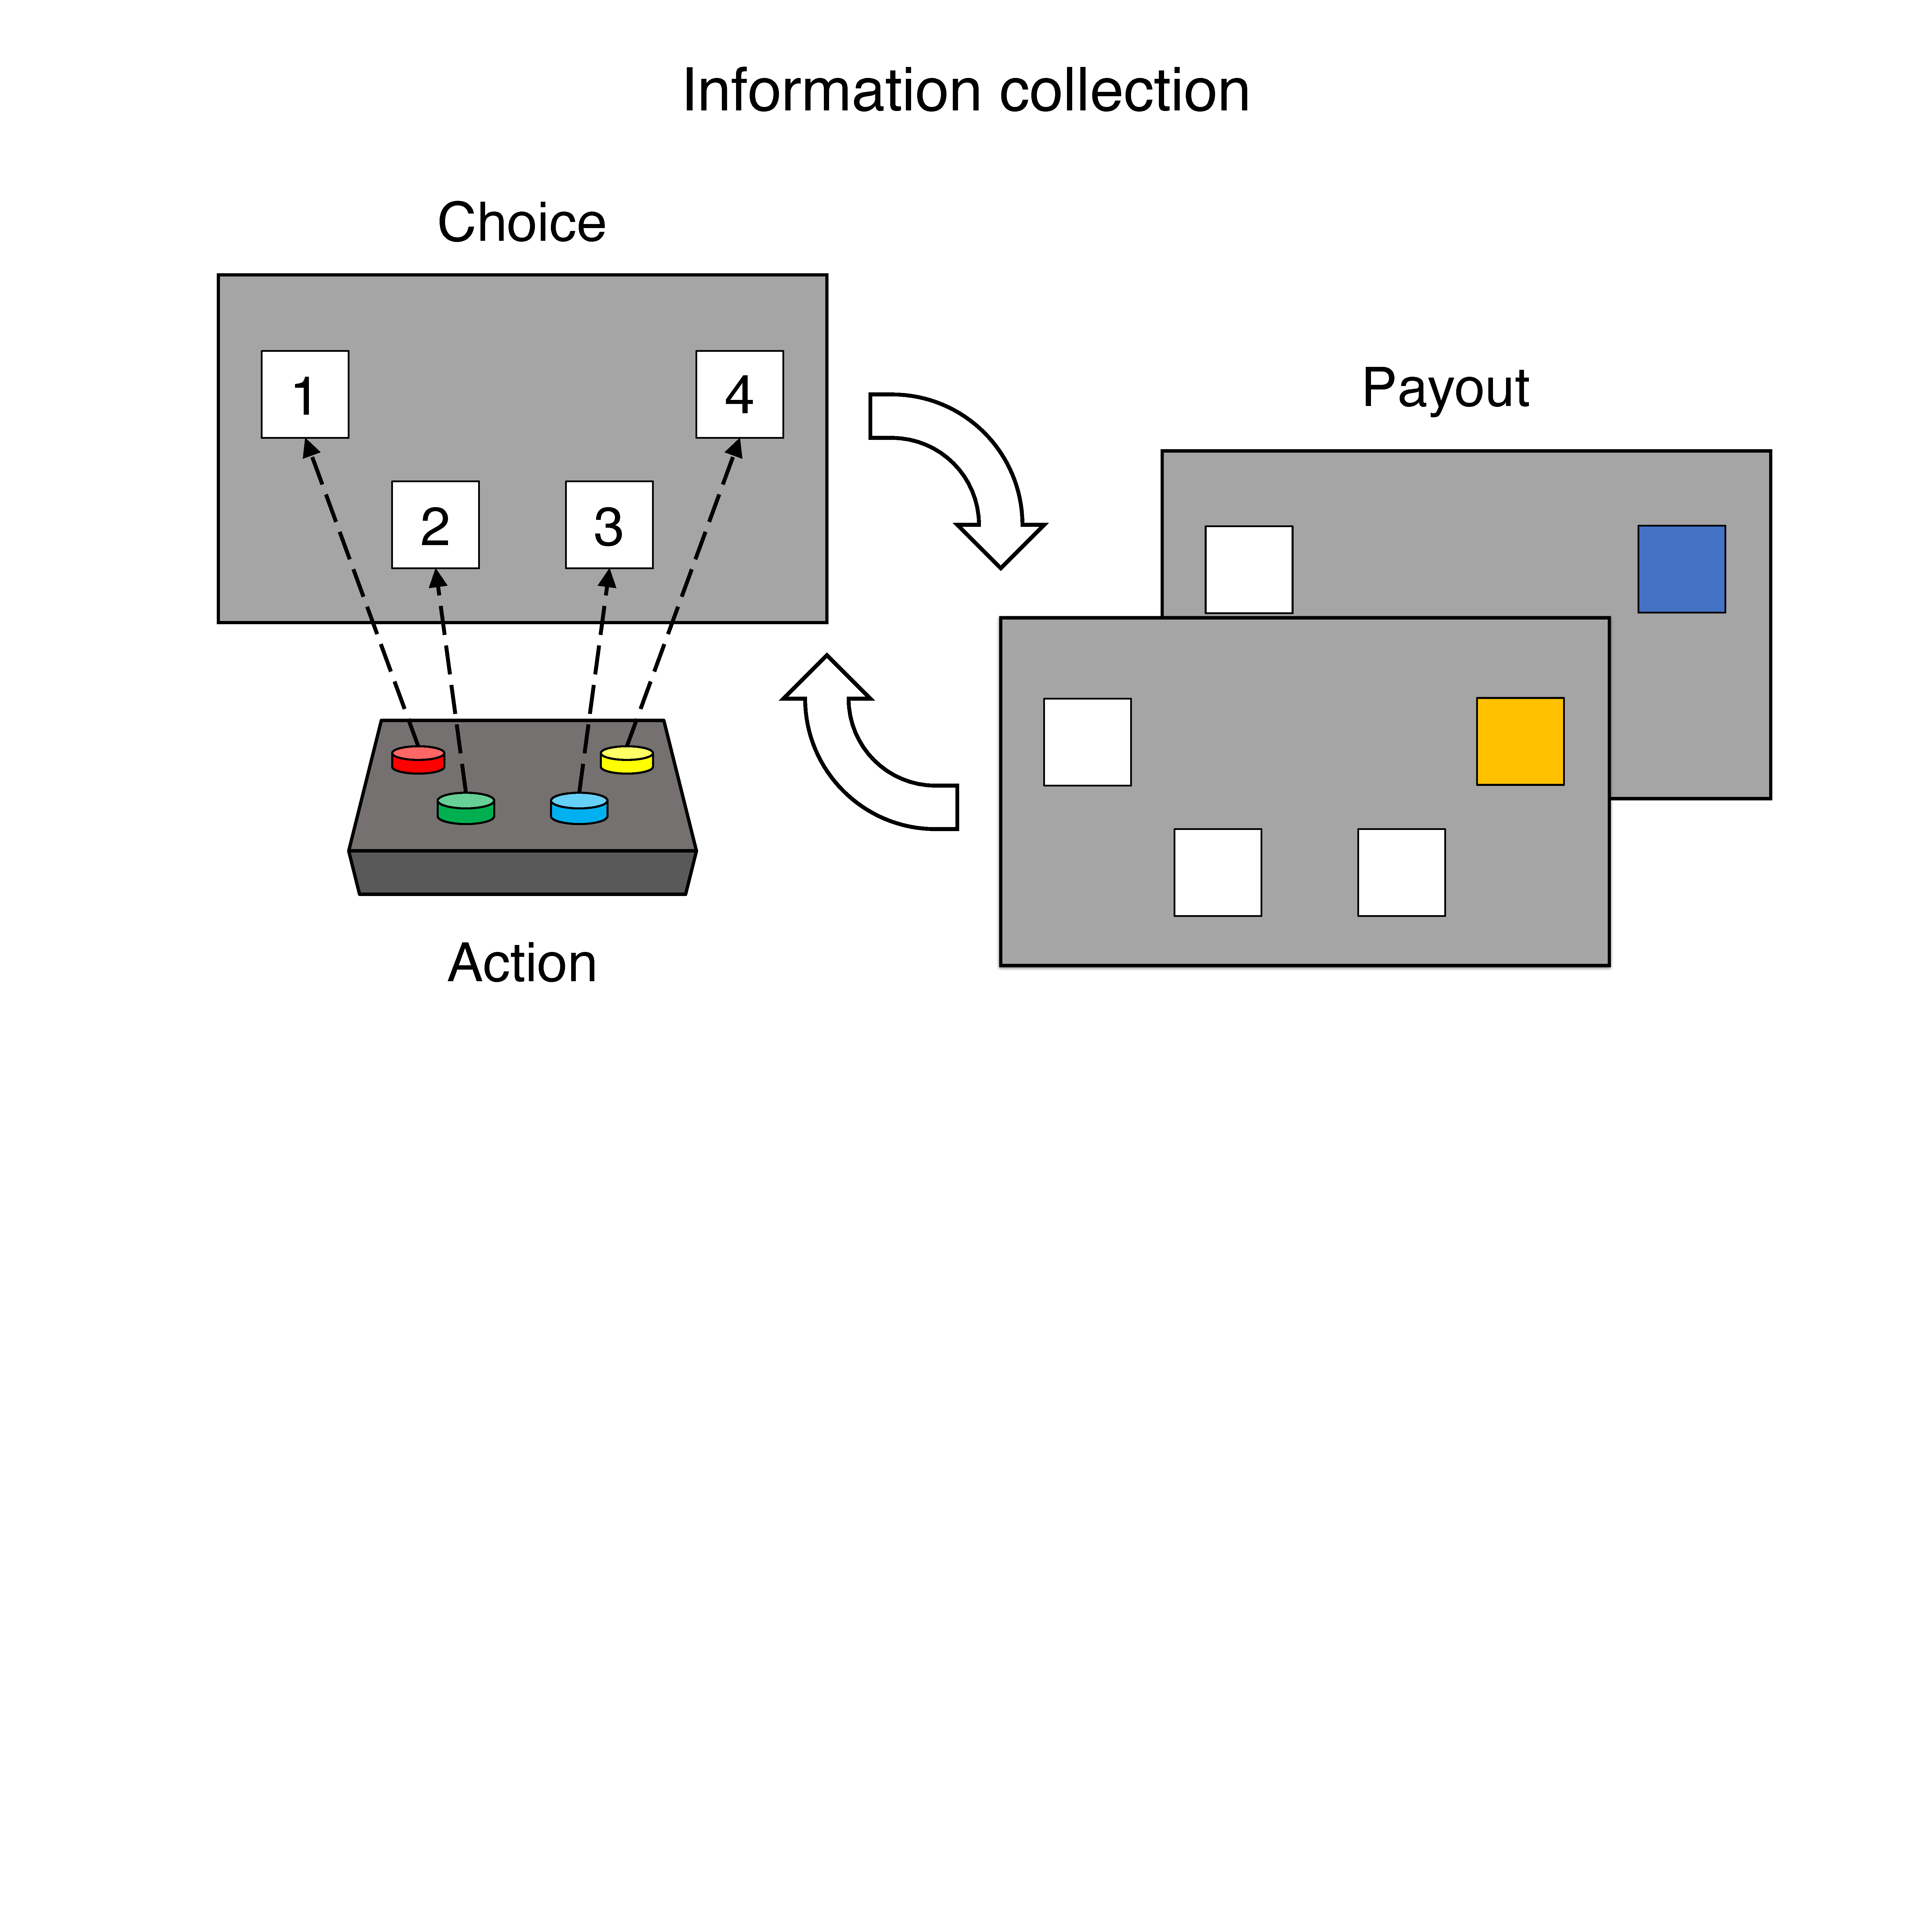
\includegraphics[width=.55\linewidth]{img/task_outline1.pdf} 
	\caption{A simple four choice information foraging task. The information in this task is a yellow or blue stimulus, which can change from trial to trial. A good learner in this task is one who tries to learn the probabilities of all the symbols in each of the four choices. The more random the stimuli are in a choice, the more potential information/entropy there is to learn. \textit{Note}: the information payout structure is shown below (Fig.~\ref{fig:payout}a}).
	\label{fig:task_outline1} 
	\end{fullwidth}
\end{figure}

\begin{figure}
	\begin{fullwidth}
	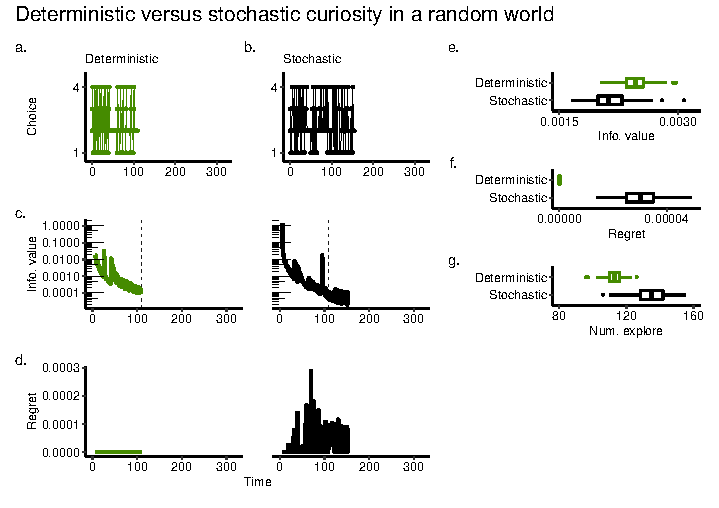
\includegraphics[width=.7\linewidth]{img/curiosity1.pdf} 
	\caption{Comparing deterministic versus stochastic variations of the same curiosity algorithm, in a simple information foraging task (Task 1). Deterministic results are shown in the left column, and stochastic are shown in the right. The hyperparameters for both models were found by random search, which is described in the Methods.
	\textbf{a-b}. Examples of choice behavior.
	\textbf{c-d}. Information value plotted with time for the behavior shown in a-b.
	\textbf{e-f}. Regret plotted with time for the behavior shown in a-b. Note how our only deterministic curiosity generates zero regret, inline with theoretical predictions.
	\textbf{e}. Average information value for 100 independent simulations. Large values mean a more efficient search.
	\textbf{f}. Average regret for 100 independent simulations. Ideal exploration should have no regret. 
	\textbf{g}. Number of steps it took to reach the boredom threshold $eta$. Smaller values imply a faster search.
	}
	\label{fig:curiosity1} 
	\end{fullwidth}
\end{figure}

\subsection{Two conjectures}
How can we justify using curiosity for the dilemma when the goal of exploitation is reward collection? Intuition suggests that this is wrong-headed. Searching in an open-ended way for information must be less efficient than a direct search. In answer to this we make two conjectures.

\begin{itemize}
	\item \textbf{Conjecture 1} Reward value and information value are equally important.
\end{itemize}

Rewards are a primary motivator for behavior in exploration \citep{Sutton2018}. Information is a primary motivator of behavior in exploration  \citep{Inglis2001}. So which view is right? We believe that trying to assess the overall worth of reward or information is a mistake. We cannot, and should not, weigh these two perspectives on the whole. They are equals. To decide between them, it is their values in the moment which matter most.

If both reward and information are equally important, then time is not wasted in a curious search and so the process is not \textit{necessarily} inefficient. The question becomes instead, is curiosity practical enough? This leads us to the next conjecture. 

\begin{itemize}
	\item \textbf{Conjecture 2} Curiosity is a sufficient solution to exploration (when learning is the goal)
\end{itemize}

We detail why this is the case in the next few sections.

\subsection{A win-stay, lose-switch solution}
If reward and information are equally important, how can an animal go about balancing them? If you accept our conjectures, then answering this last question is the same as answering the dilemma itself. 

We posit that, based on our framing of $E$, this boils down to a scheduling problem. When to shift from maximizing information to maximizing rewards, and vice versa? 

Here we propose that a win-stay, lose-switch strategy is in fact an optimal and tractable solution to this scheduling problem.

Win-stay lose-shift is a strategy famous from game theory \citep{Nowak1993}, where a player will keep its current strategy under winning conditions, and shift otherwise. We see the same kind of patterning as useful here, except the ``players'' are two different policies inside the animal. They are competing for behavioral control. Imagine that in the previous action our bee from Fig. ~\ref{fig:bee} observed 0.7 units of information value, $E$, and no reward (i.e. 0). Using our rule on the next action, the bee should then choose its exploration policy. Let us say that this time $E$ decreases to 0.6, and a reward value of 1.0 is observed. Now the bee should change its strategy for the next round, to exploit instead. In general then if there was more reward value then information value last round ($R_{t-1} > E_{t-1}$), our rule dictates an animal should choose the reward policy. If information value dominated, $E_{t-1} >\ge R_{t-1}$, then it should choose the information gathering policy.

To prove the optimality of our rule we will use regret minimization, which is a standard metric of optimality in reinforcement learning \citep{Sutton2018}. Regret is a numerical quantity of the difference between the most valuable choice and the value of the choice that was made. To approximate regret $G$ we use Eq.~\ref{eq:regret}, where $V$ is the value of the chosen action, and $V^*$ is the maximum value. 

\begin{equation}
\label{eq:regret}
	G = V^* - V
\end{equation}

An optimal value algorithm always makes the most valuable choice. It therefore will have zero regret, by Eq.~\ref{eq:regret}. This is impossible to achieve, of course, using stochastic search. To find the algorithm that maximizes both information and reward value with zero regret, we therefore need a deterministic method. 

To prove things about our solution we will move from game theory, which gave us our inspiration, to the field of optimal scheduling \citep{Bellmann1954,Roughgarden2019}. Put another way, we will now answer the question, when does win-stay, lose-switch strategy work as an optimal scheduler? 

We imagine the policies for exploration and exploitation acting as two possible ``jobs'' competing for control of behavior, a fixed resource. We know by definition that each of these jobs produces non-negative values which an optimal job scheduler could use: $E$ for information or $R$ for reward/reinforcement learning. We can also ensure, again by definition, that each of the jobs takes a constant amount of time and that each policy can only take one action at a time. These two properties, and one further assumption, are sufficient.

We believe it is also reasonable to assume that there will be no model of the environment available to the learner at the start of a problem, and that its environment is nonlinear but deterministic. 

We arrived at our solution by taking the simplest possible path available. We just wrote down the simplest equation that could have zero regret answer, and began to study that. This is Eq.~\ref{eq:meta_greedy}. We refer to it as a meta-greedy algorithm, as it decides in greedy fashion which of our independent policies to use.

\begin{equation}
\label{eq:pipi} 
\pi^{\pi} = \ \Big [ \pi_E,\ \pi_R \Big ]
\end{equation}

\begin{equation}
\label{eq:meta_greedy} 
	\argmax_{\pi^{\pi}} \ \Big [ E_{t-1} - \eta,\ R_{t-1} \Big ]_{\textbf{(2, 1)}}
\end{equation}
	
We have modified traditional argmax notation in Eq. \ref{eq:meta_greedy}. It now includes a subscript vector, $(2,1)$ to denote a ranking for which value/policy should be preferred in the event of a tie. Smaller numbers are preferred. We did this because an exact rule for tie breaking is critical for our proofs. In Eq. \ref{eq:meta_greedy} we also limit the probability of having zero reward to be, itself, non-zero. That is, $p(R_t=0) > 0$. We also limit $E_0$, the first set of values, to be positive and non-zero when used with boredom, $(E_0 - \eta) \geq 0$. Both are necessary to ensure exploration. 

In Theorem \ref{theorem:meta_total} we prove Eq. \ref{eq:meta_greedy} is Bellman optimal, and so it will always find a maximum value sequence of $E$ and $R$ values. Given, that is, that the environment is deterministic. In Theorem \ref{theorem:meta} we also prove that with a judicious choice in boredom $\eta$, the reward policy $\pi_R$ will also converge to its optimal value, assuming that it has one. Full details for these proofs are found in the mathematical appendix.


% -------------------------------------------------------------------------
\begin{featurebox}
	\caption{Reward homeostasis.}
	\label{box:complexity}
	We have been studying a kind of reinforcement learning where the value of a reward is fixed. We'll call this the economic style. It is the most common kind of model found in machine learning, psychology, neuroeconomics, and neuroscience \citep{Sutton2018}. In natural behavior though it is common that the motivational value of reward declines as the animal gets ``full'', or reaches satiety. We'll call this the homeostatic style \citep{Keramati2014,Juechems2019,Munch2020}.
	Fortunately it has already been proven that a reward collection policy designed for one style will work for the other (at least this is so an infinite time-horizon \citep{Keramati2014}). However to use Eq. \ref{eq:meta_greedy} for reward homeostasis requires that we make one modification. Ties between values should be broken in favor of exploration, and information seeking. This is in contrast to the economic reinforcement learning approach where ties break in favor of exploiting rewards. This modification leads to Eq. \ref{eq:meta_greedy_h}.

	\begin{equation}
		\label{eq:meta_greedy_h} 
			\argmax_{\pi^{\pi}} \ \Big [ E_{t-1},\ R_{t-1} \Big ]_{\textbf{(1, 2)}}
		\end{equation}
	\medskip
\end{featurebox}
% -------------------------------------------------------------------------

\subsection{Reward collection} We will now focus on practical performance in reward collection. The general form of the 7 tasks we will study is depicted in Fig~\ref{fig:task_outline2}. As with our first task (Fig. ~\ref{fig:task_outline1}) they are all variations of the classic multi-armed bandit \citep{Sutton2018}. The payouts for each of the tasks are shown separately in Fig.~\ref{fig:payout}. Each was designed to either test exploration performance in a way that matches recent experimental study(s), or to test the limits of curiosity. Every trial has a set of $n$ choices. Each choice returns a “payout”, according to a predetermined probability. Payouts are information, a reward, or both. Note that, as in Task 1, information was symbolic, denoted by a color code, “yellow” and “blue” and as is custom reward was a positive real number. 
To evaluate the performance of our curiosity algorithm, we compare it against a range of other exploration strategies found in the literature. For a brief description of each, see Table~\ref{tab:agents}. We feel this set is a broad and fair representation of today's state-of-the-art approaches.

They all have in common that their central goal is to maximize reward value, though this is often supplemented by some other goal.  The results in full for all tasks and exploration strategies are shown in Fig.~\ref{fig:summary}. All learners, including ours, used the same exploitation policy, based on the temporal difference learning rule \citep{Sutton2018}.

\begin{figure}
	\begin{fullwidth}
	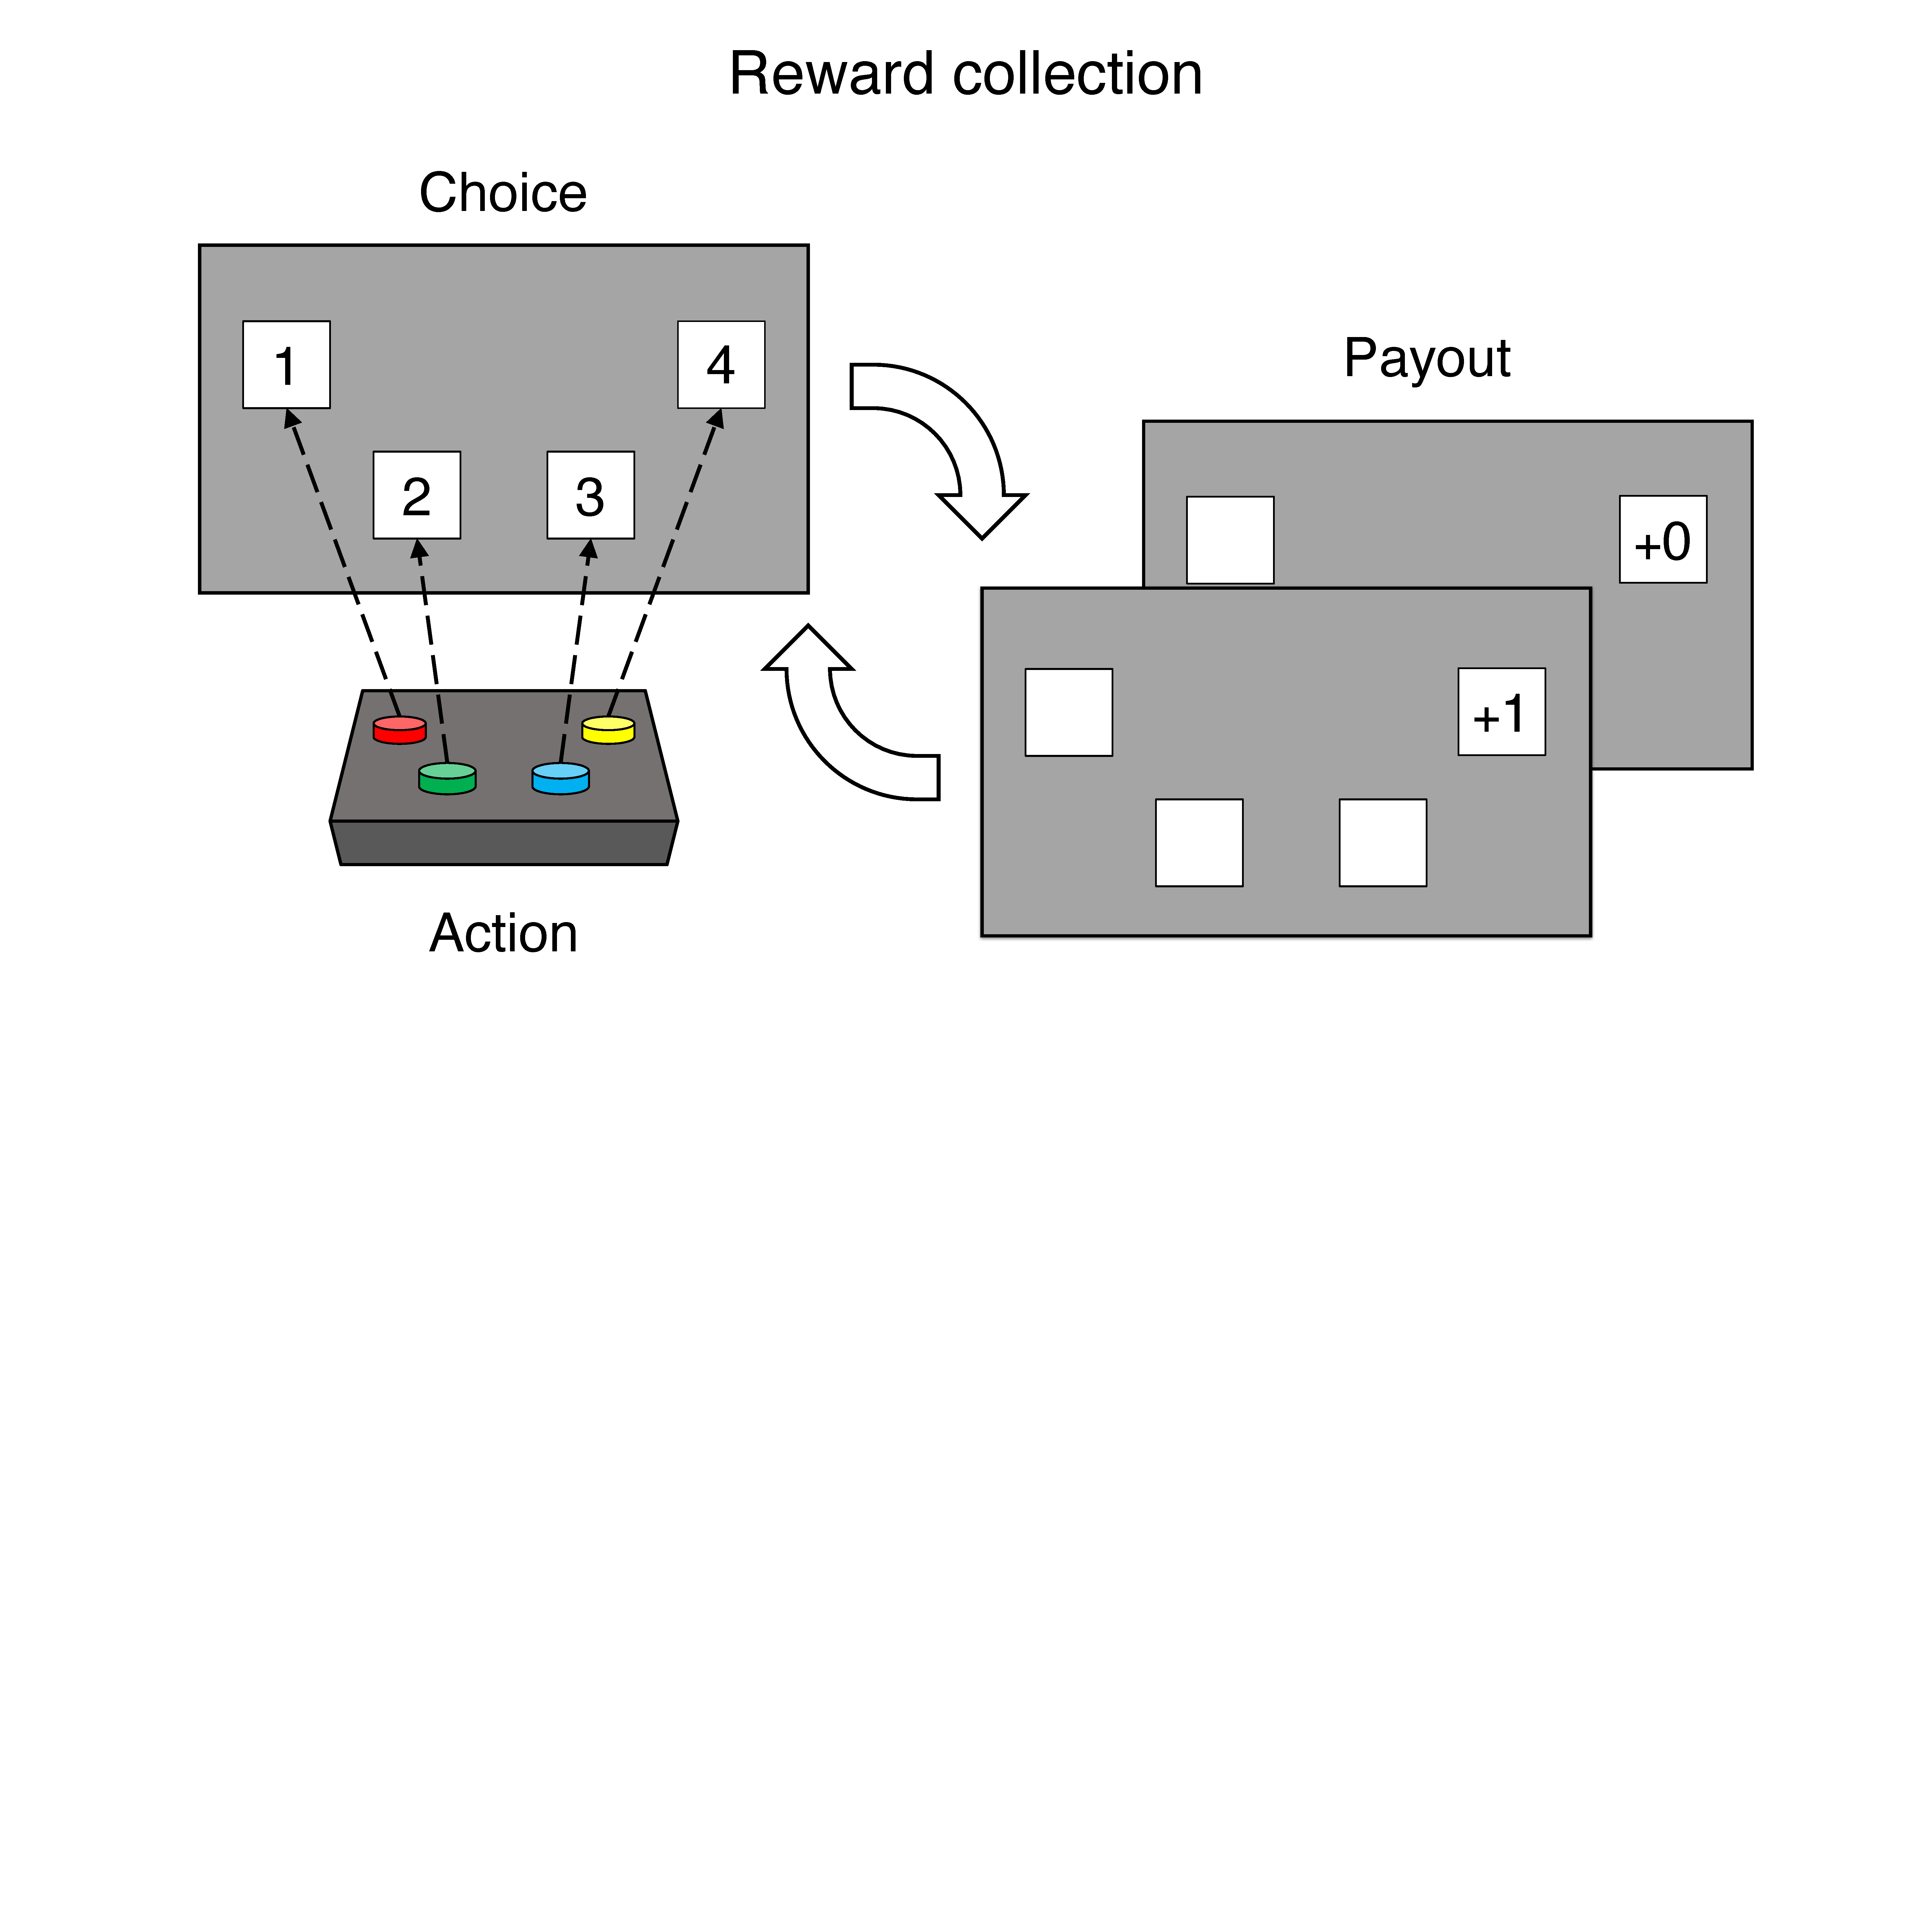
\includegraphics[width=.55\linewidth]{img/task_outline2.pdf} 
	\caption{A 4 choice reward collection task. The reward is numerical value, here a 1 or 0. A good learner in this task is one who collects the most rewards. The task depicted here matches that in Fig~\ref{fig:payout}b. Every other reward collection task we study has the same basic form, only the number of choices increases and the reward spaces are more complex.}
	\label{fig:task_outline2} 
	\end{fullwidth}
\end{figure}

\begin{figure}
	\begin{fullwidth}
	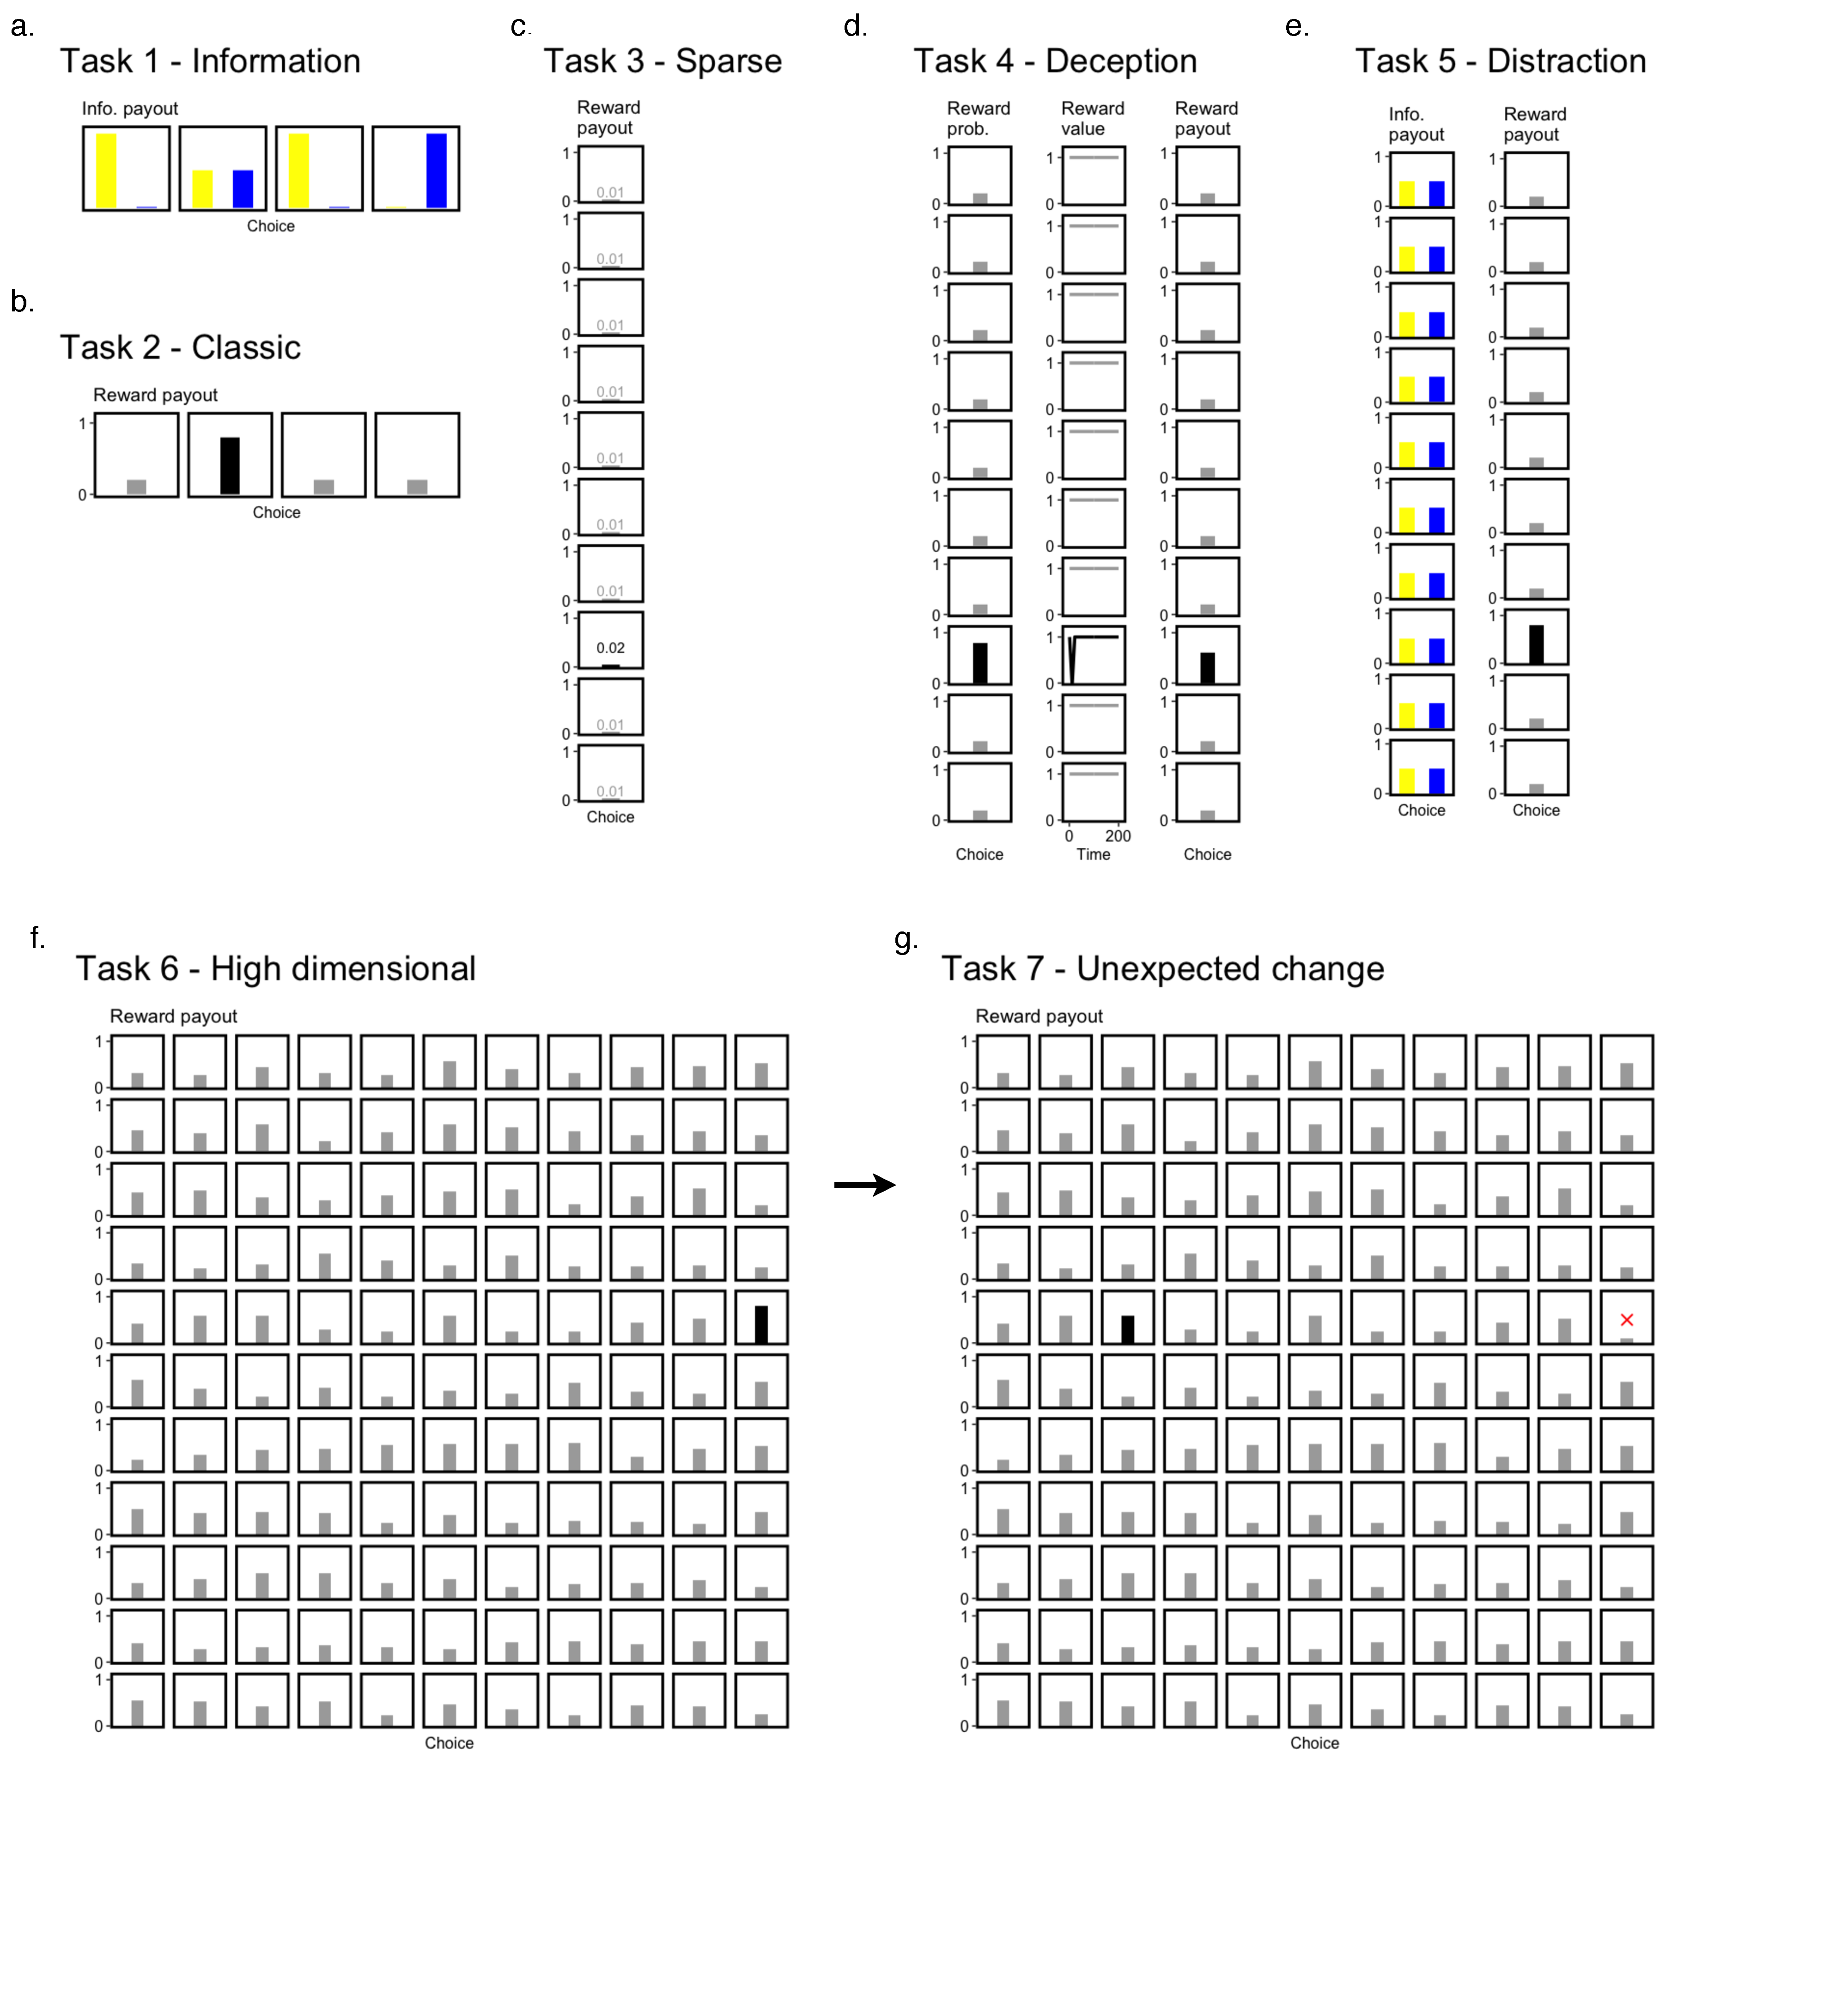
\includegraphics[width=0.9\linewidth]{img/task_payout.pdf} 
	\caption{Payouts for \textit{Tasks 1 - 7}. Payouts can be information, reward, or both. For comments on general task design, see Fig~\ref{fig:task_outline2}.
	\textbf{a.} A classic four-choice design for information collection. A good learner should visit each arm, but quickly discover that only arm two is information bearing.
	\textbf{b.} A classic four-choice design for testing exploration under reward collection. The learner is presented with four choices and it must discover which choice yields the highest average reward. In this task that is Choice 2. 
	\textbf{c.} A ten choice sparse reward task. The learner is presented with four choices and it must discover which choice yields the highest average reward. In this task that is Choice 8 but the very low overall rate of rewards makes this difficult to discover. Solving this task with consistency means consistent exploration. 
	\textbf{d.} A ten choice deceptive reward task. The learner is presented with 10 choices, but the choice which is the best on the long-term (>30 trials) has a lower value in the short term. This value first declines, then rises (see column 2).
	\textbf{e.} A ten choice information distraction task. The learner is presented with both information and rewards. A good learner though will realize the information does not predict reward collection, and so will ignore it.
	\textbf{f.} A 121 choice task with a complex payout structure. This task is thought to be at the limit of human performance. A good learner will eventually discover choice number 57 has the highest payout.
	\textbf{g.} This task is identical to \textit{a.}, except for the high payout choice being changed to be the lowest possible payout. This task tests how well different exploration strategies adjust to simple but sudden change in the environment.
	}
	\label{fig:payout} 
	\end{fullwidth}
\end{figure}

\begin{table}[]
	\caption{Exploration strategies.}
	\label{tab:agents}
	\begin{tabular}{|l|l|l|}
	\hline
	\textbf{Name} & \textbf{Class} & \textbf{Exploration strategy} \\ \hline
	Curiosity & Deterministic & Maximize information value \\ \hline
	Random/Greedy & Random & \begin{tabular}[c]{@{}l@{}}Alternates between random exploration \\ and greedy with probability $\epsilon$.\end{tabular} \\ \hline
	Decay/Greedy & Random & \begin{tabular}[c]{@{}l@{}}The $\epsilon$ parameter \\ decays with a half-life $\tau$\end{tabular} \\ \hline
	Random & Random & Pure random exploration \\ \hline
	Reward & Extrinsic & Softmax sampling of reward value \\ \hline
	Bayesian & Extrinsic + Intrinsic & Sampling of reward value + information value \\ \hline
	Novelty & Extrinsic + Intrinsic & Sampling of reward value + novelty signal \\ \hline
	Entropy & Extrinsic + Intrinsic & Sampling of reward value + action entropy \\ \hline
	Count (EB) & Extrinsic + Intrinsic & Sampling of reward value + visit counts \\ \hline
	Count (UCB) & Extrinsic + Intrinsic & Sampling of reward value + visit counts \\ \hline
	\end{tabular}
\end{table}

\begin{figure}
    \label{fig:summary} 
	\begin{fullwidth}
	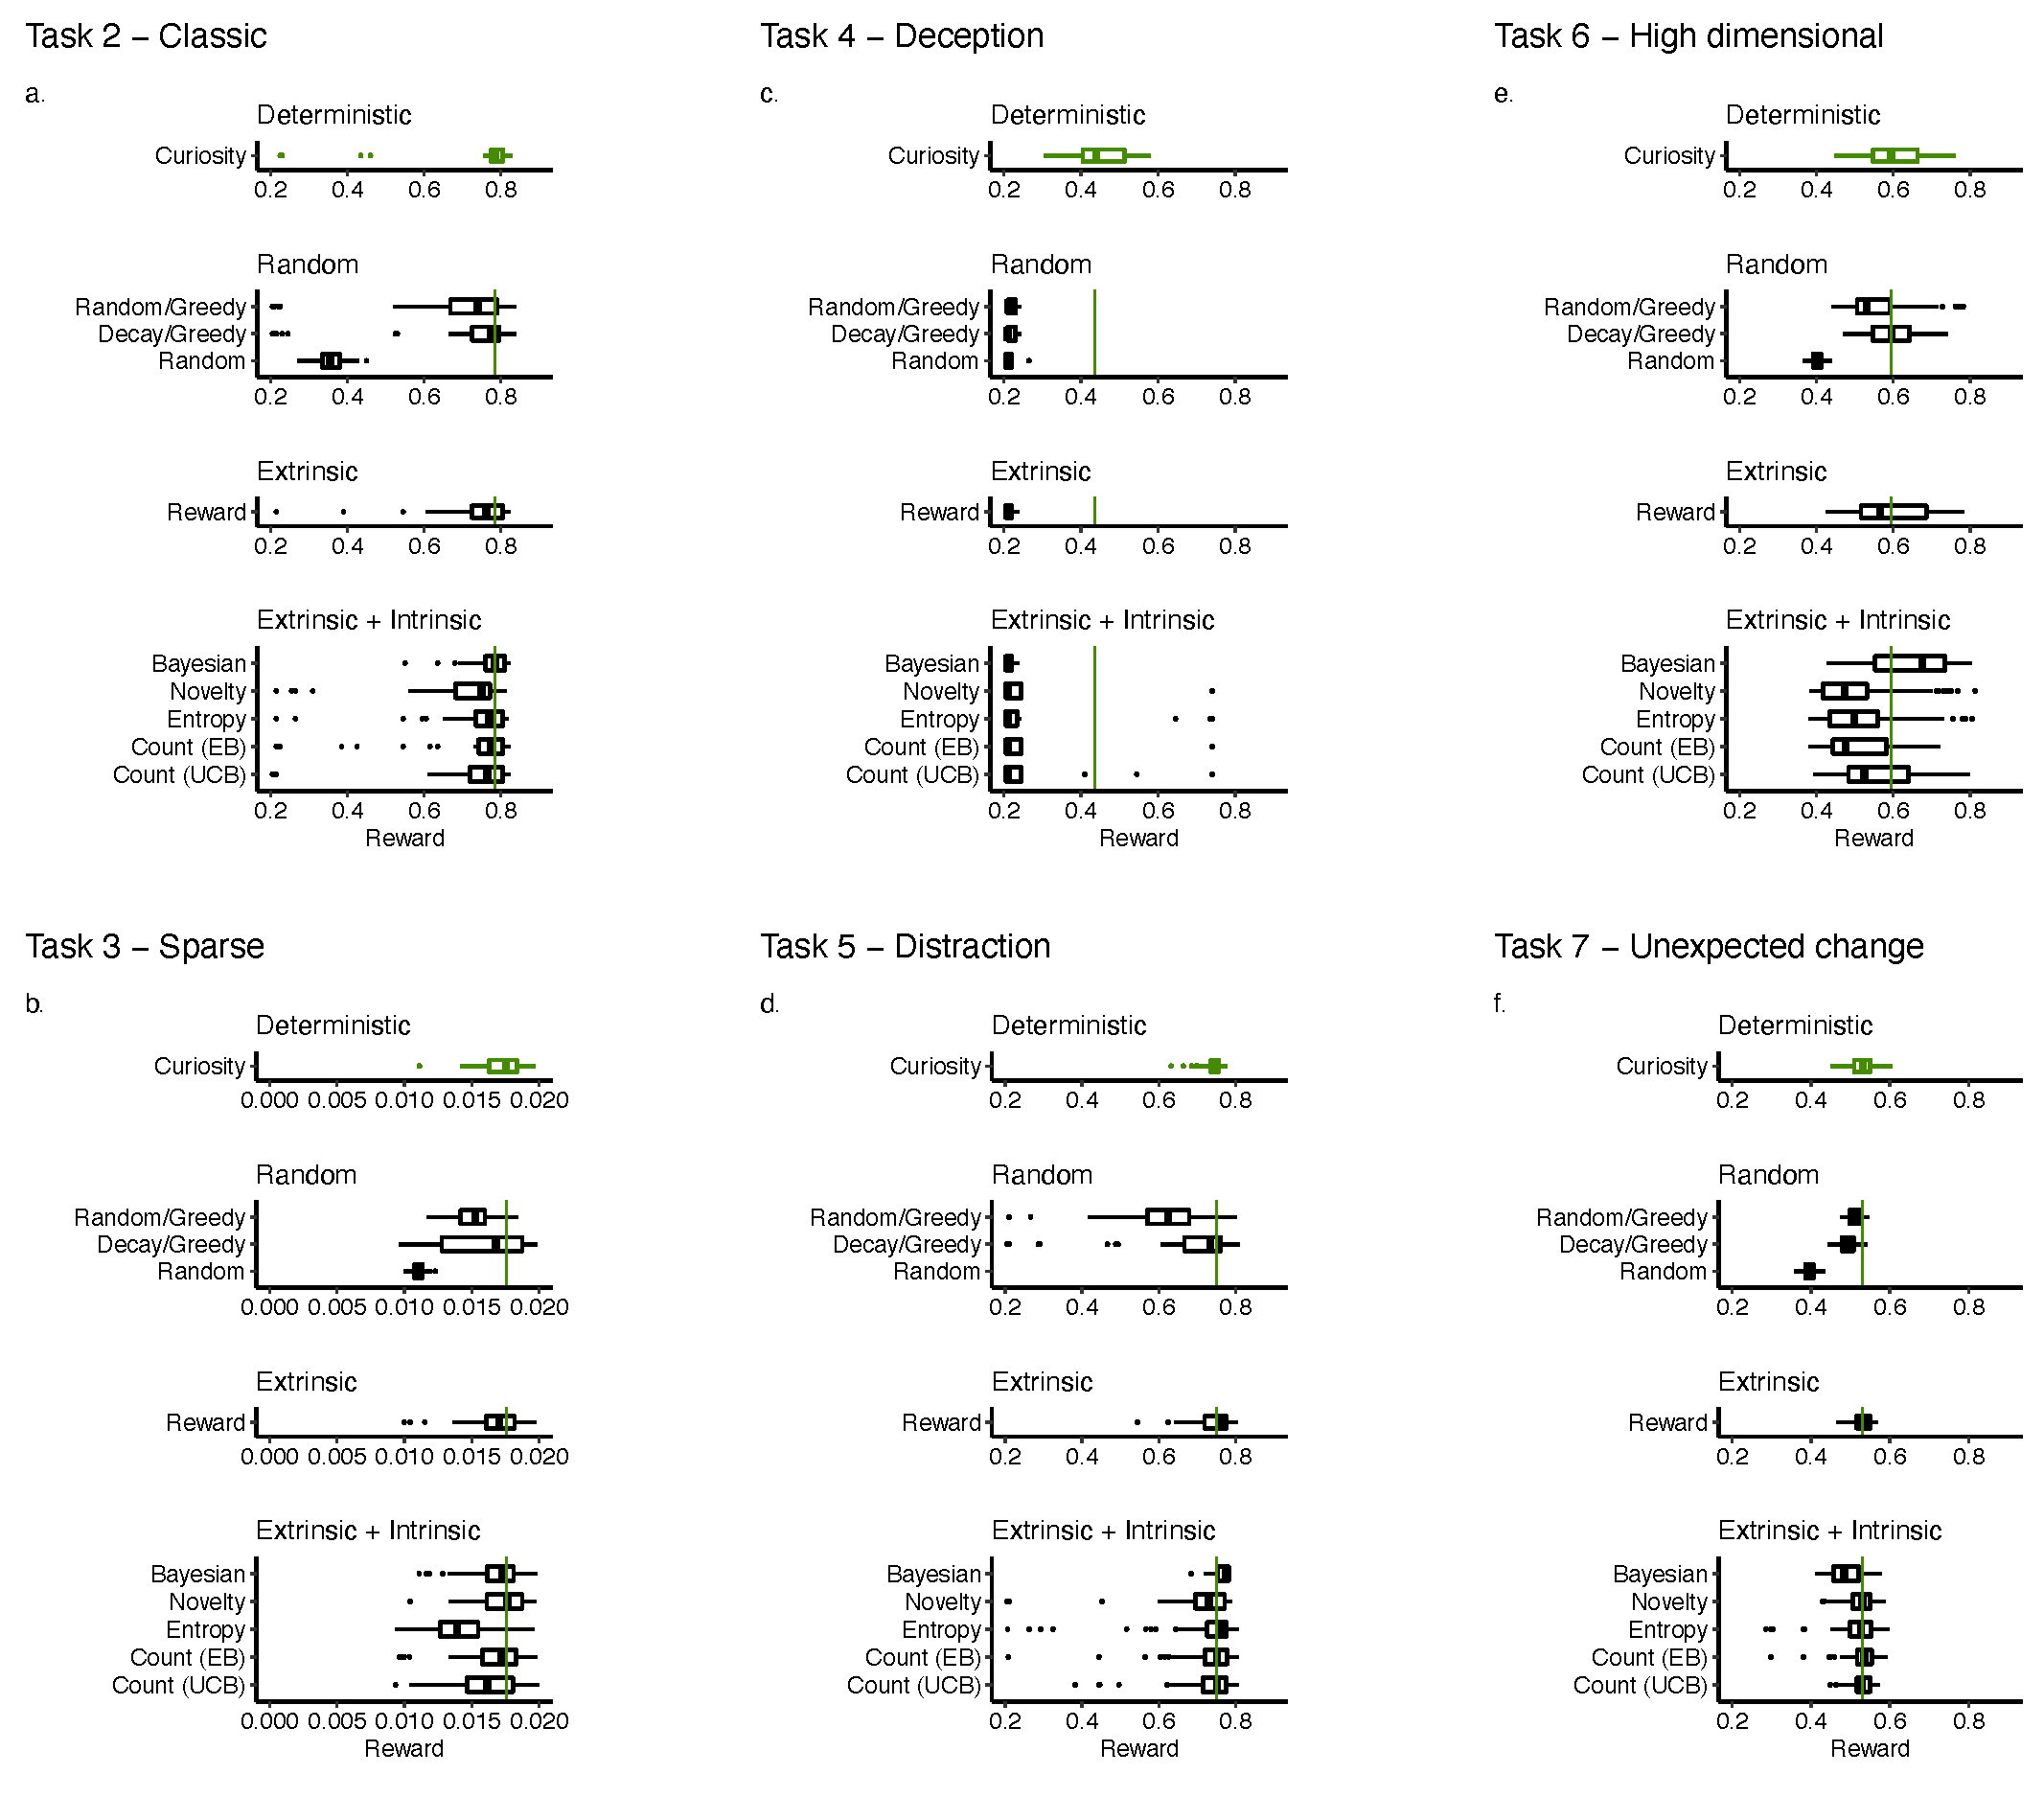
\includegraphics[width=1\linewidth]{img/summary.pdf} 
	\caption{Summary of reward collection (\textit{Tasks 2-7}). The strategies in each panel are grouped according to the class of search they employed (Curiosity. Random, Extrinsic reward or Extrinsic + Intrinsic rewards). 
	\textbf{a.} Results for Task 2, which has four choices and one clear best choice.
	\textbf{b.} Results for Task 3, which has 10 choices and very sparse positive returns.
	\textbf{c.} Results for Task 4, whose best choice is initially ``deceptive'' in that it returns suboptimal reward value over the first 20 trials.
	\textbf{d.} Results for Task 5, which blends the information foraging task 1 with a larger version of Task 2. The yellow/blue stimuli are a max entropy distraction which do not predict the reward payout of each arm.
	\textbf{e.} Results for Task 6, which has 121 choices and a quite heterogeneous set of payouts but still with one best choice.
	\textbf{f.} Results for Task 7, which is identical to Task 6 except the best choice was changed to be the worst. The learners from Task 6 were trained on this Task beginning with the learned values from their prior experience -- a test of robustness to sudden change in the environment. 
	\textit{Note}: To accommodate the fact that different tasks were run different numbers of trials, we normalized total reward by trial number. This lets us plot reward collection results for all tasks on the same scale.
  	}
	
	\figsupp{Summary of regret (\textit{Tasks 2-7})}{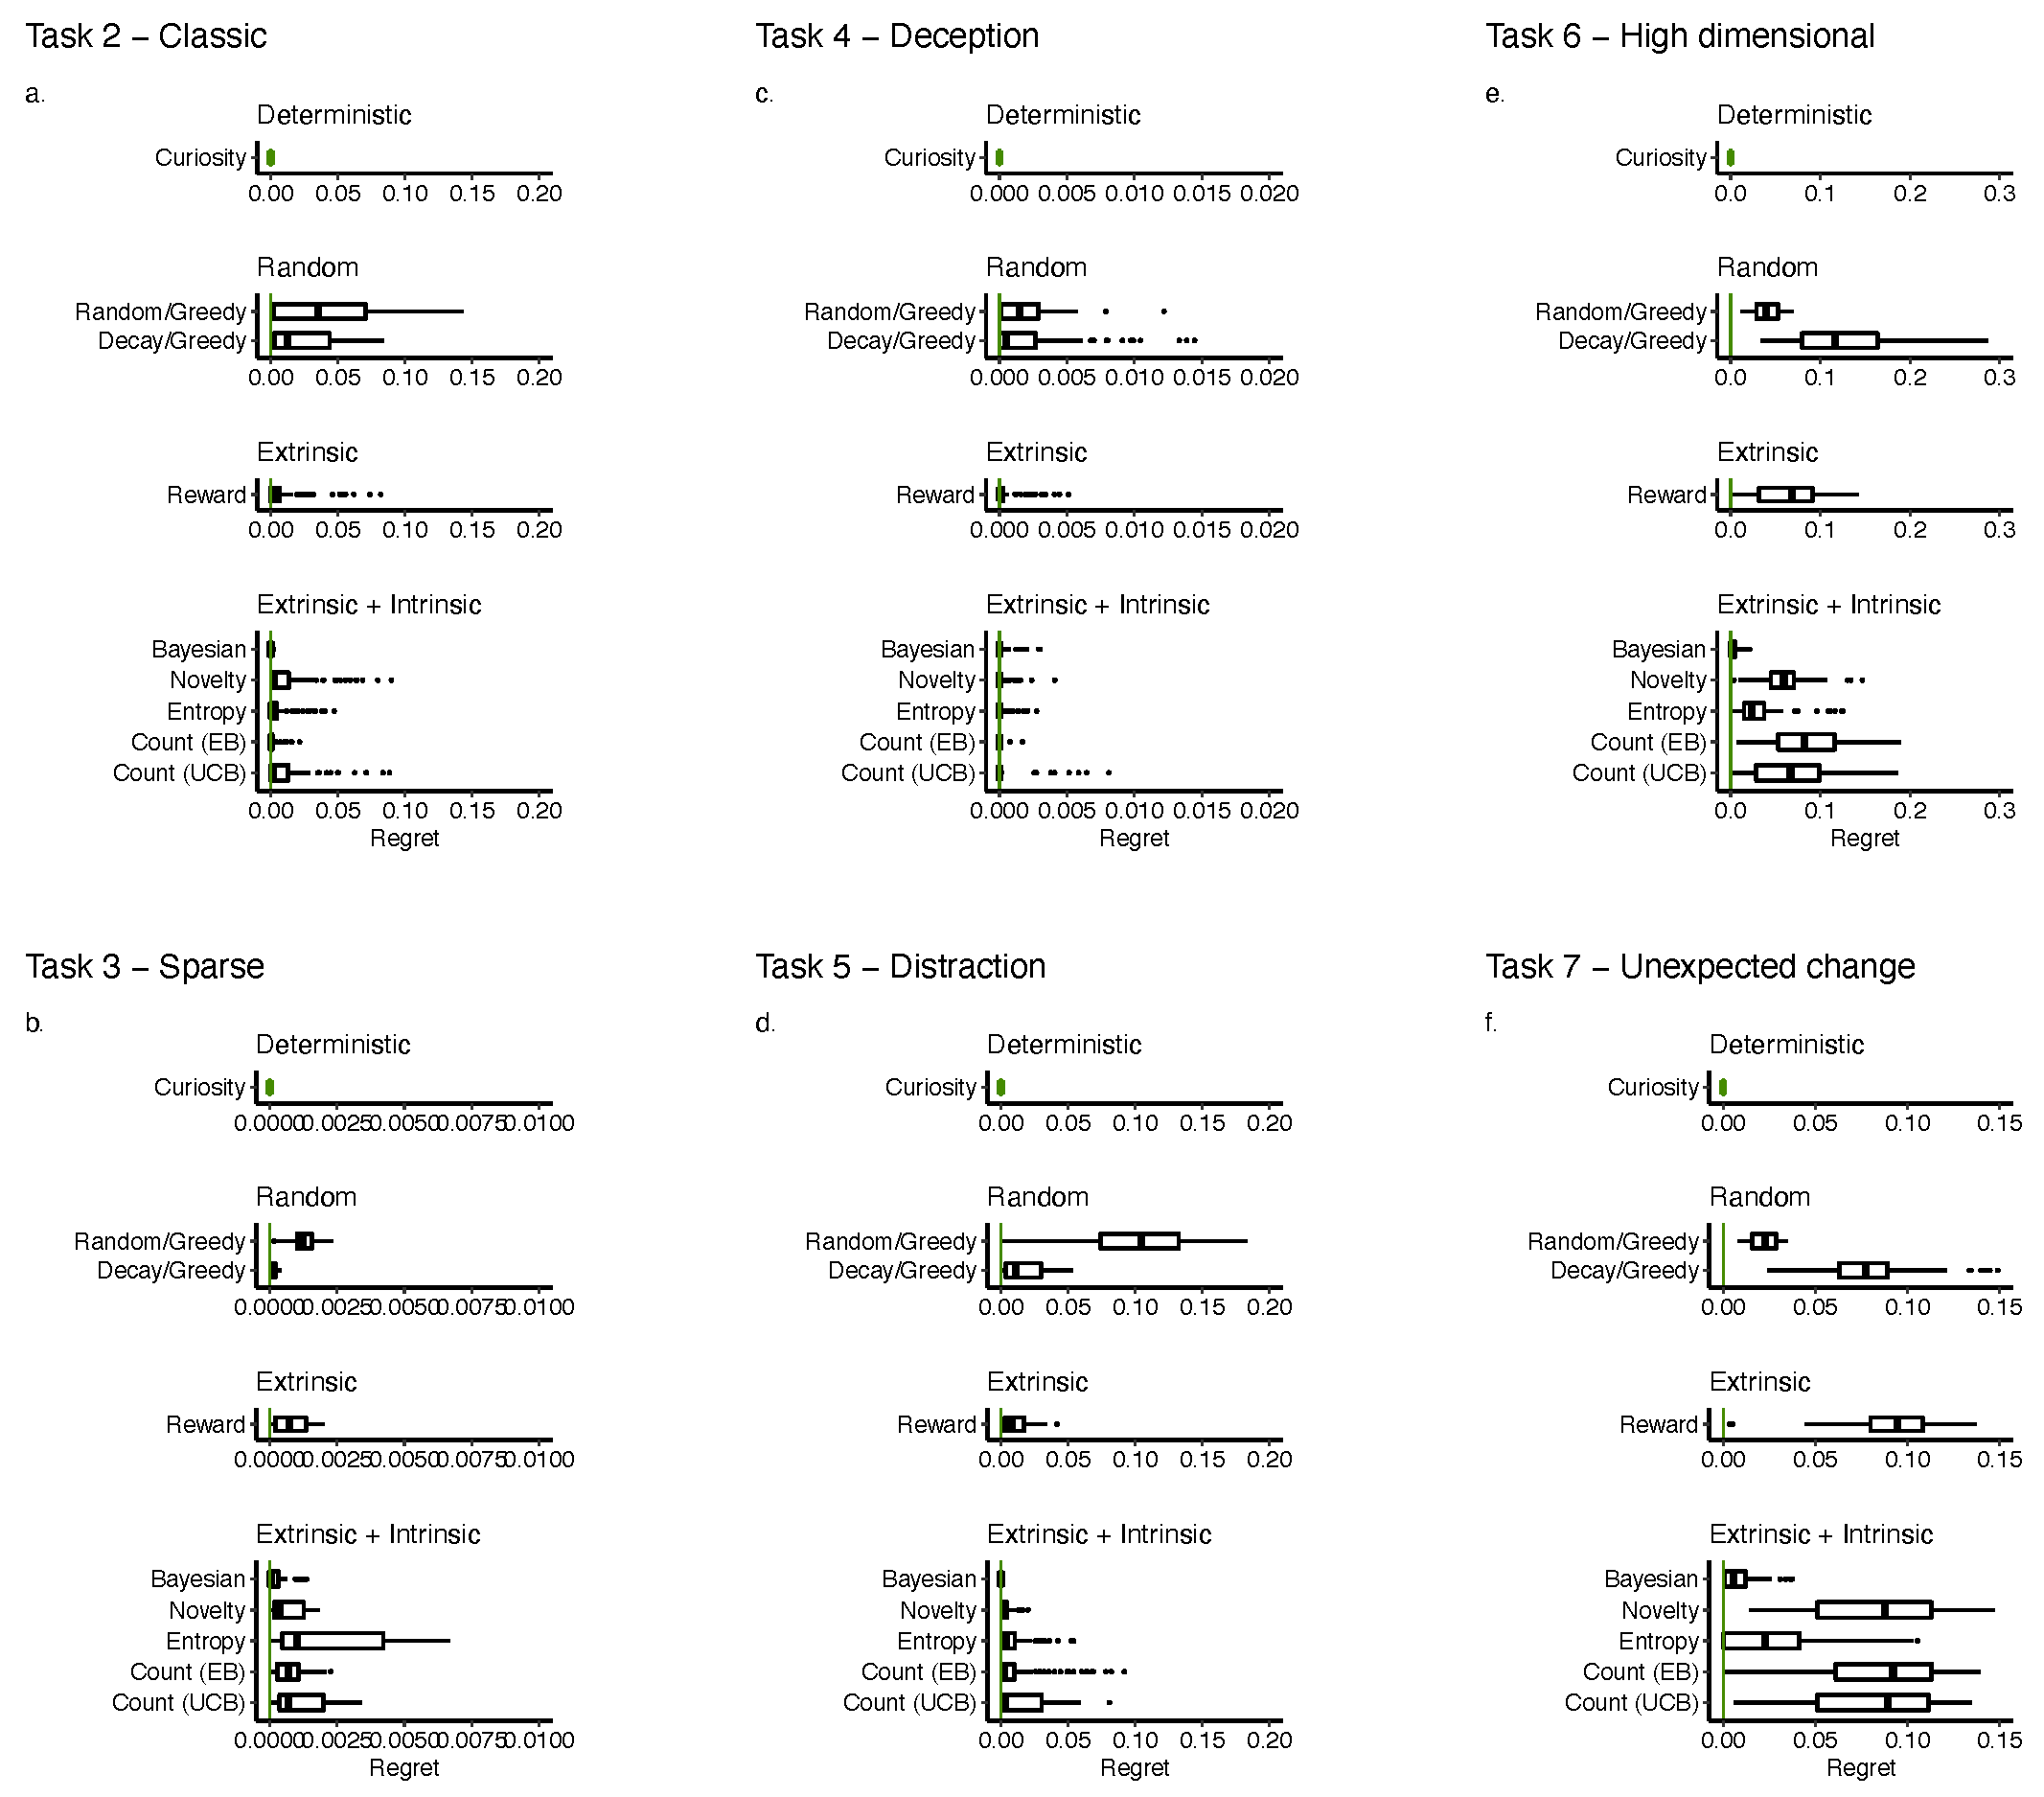
\includegraphics[width=1\linewidth]{img/supp_regret.pdf}}
	\figsupp{Summary of information value (\textit{Tasks 2-7})}{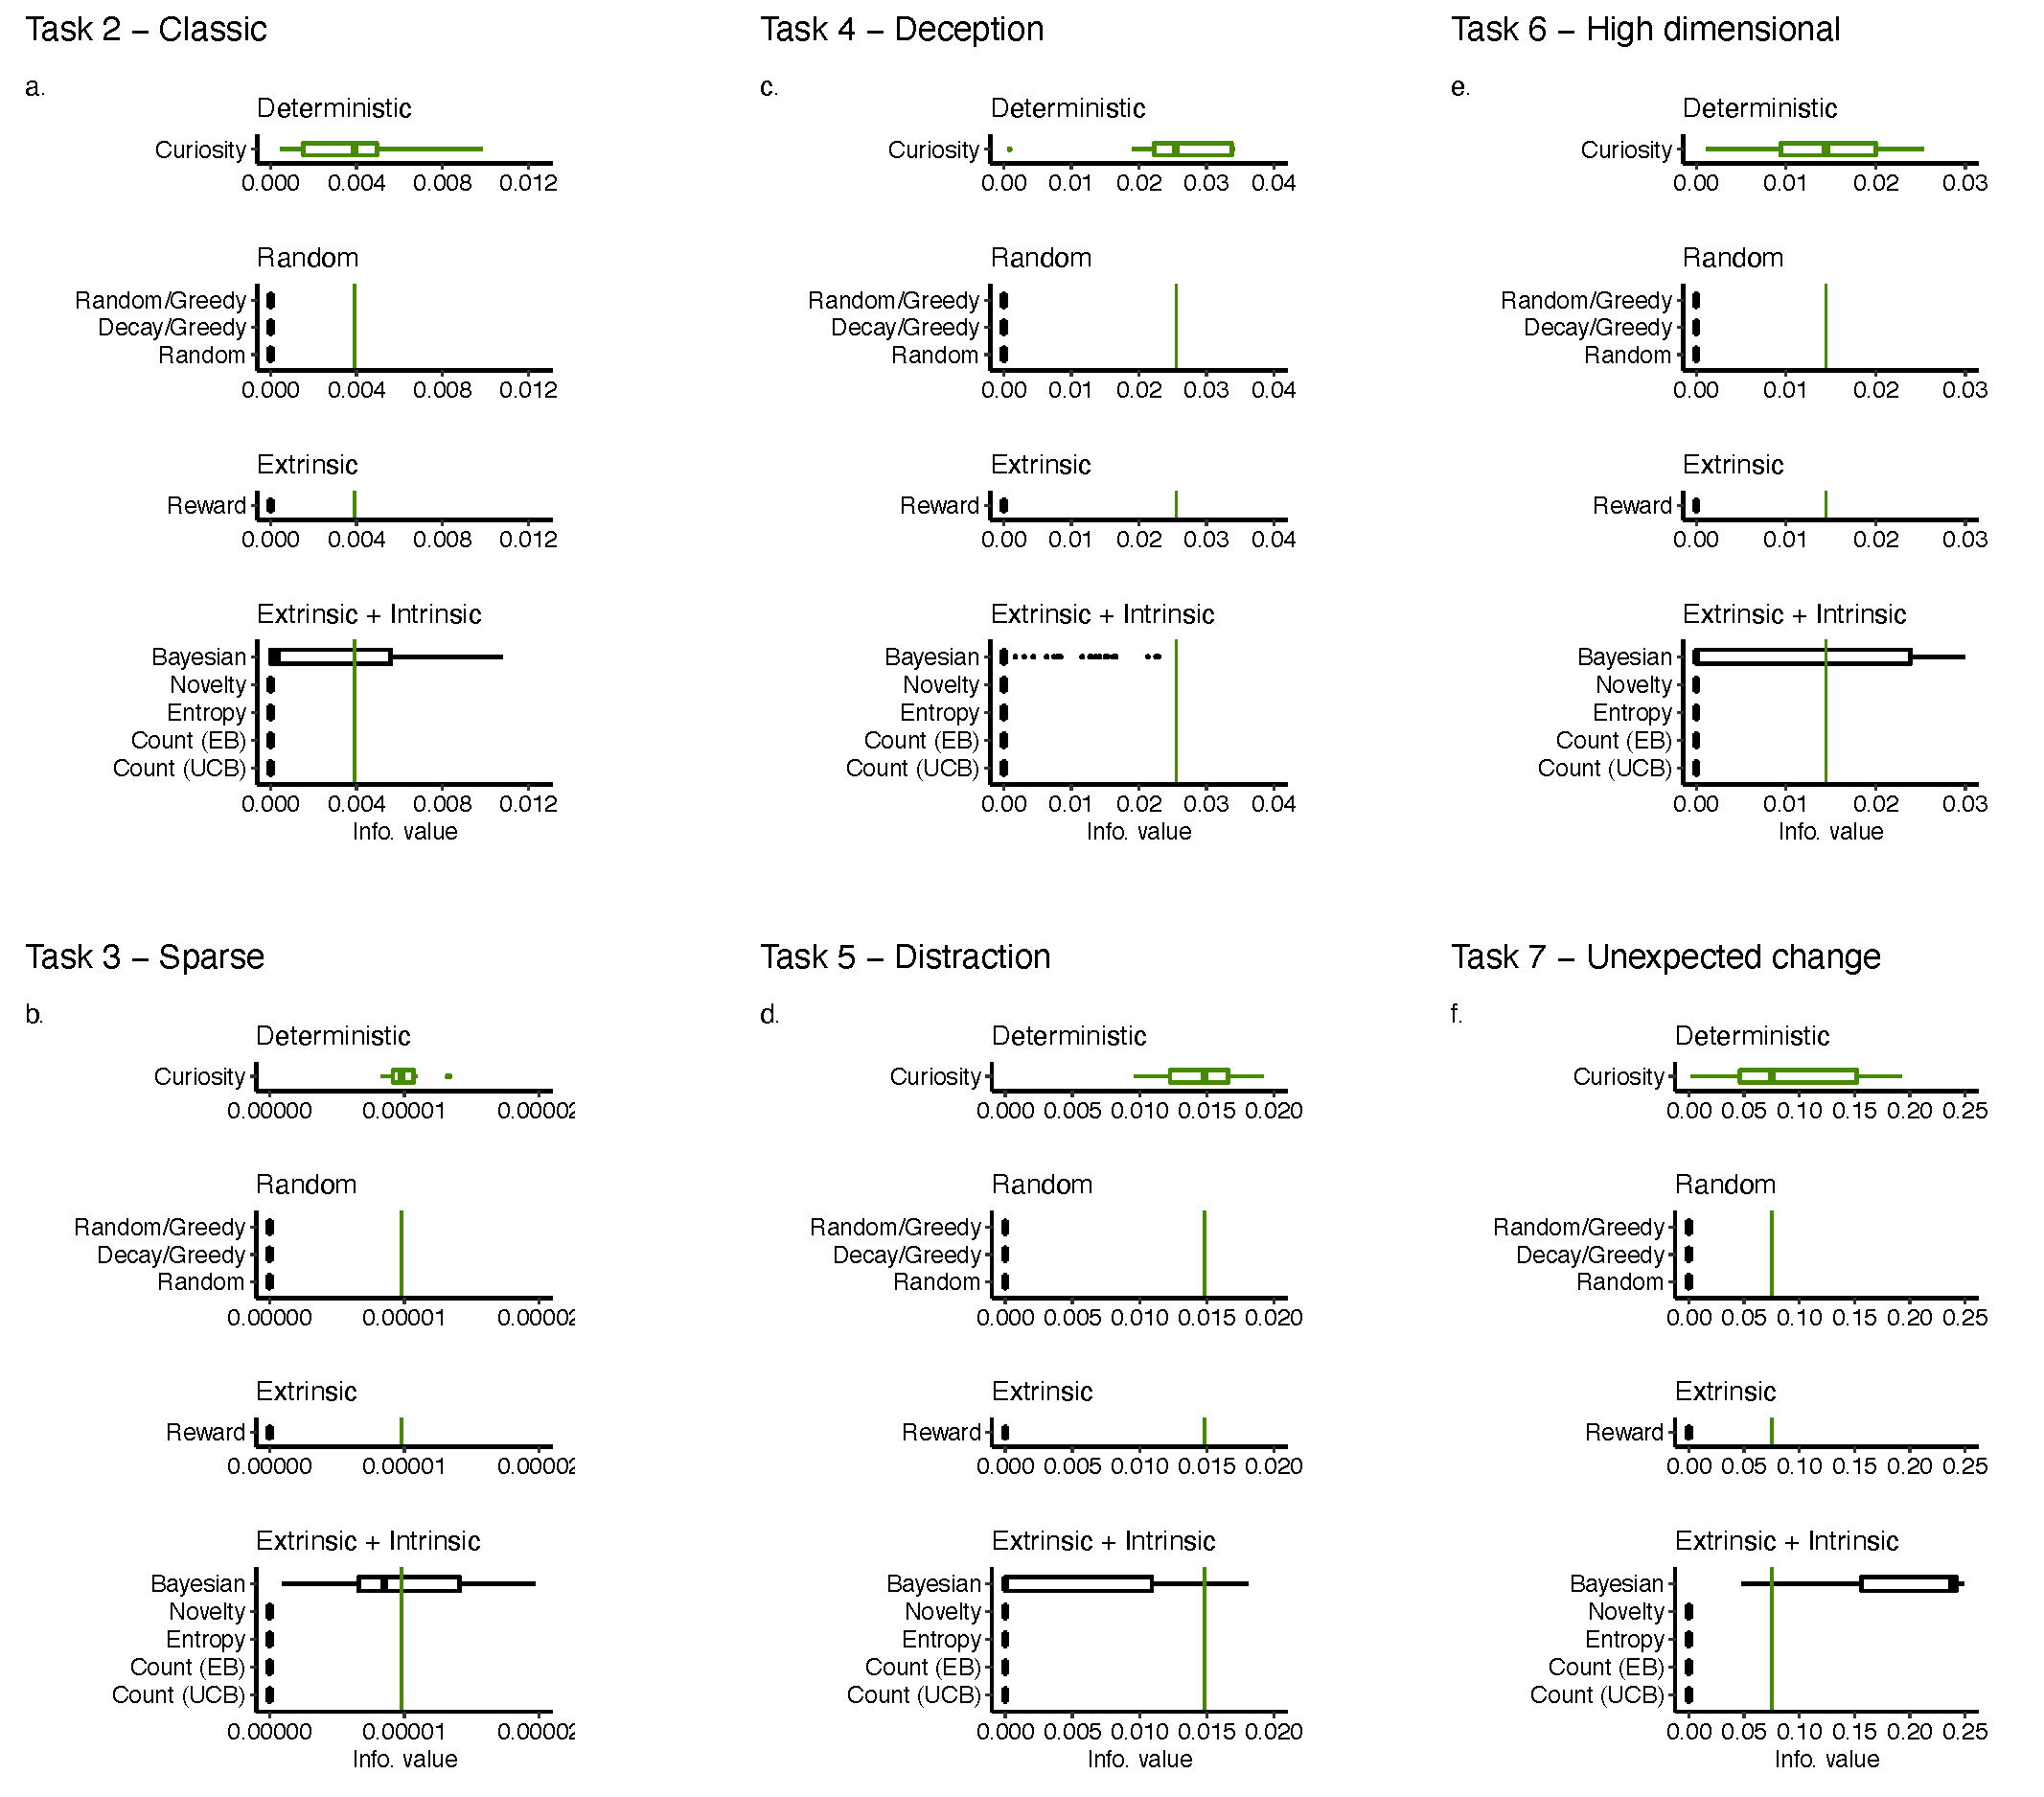
\includegraphics[width=1\linewidth]{dilemma-draft-elife/img/supp_info.pdf}}
	\figsupp{Examples of exploration (Task 1). Here we simulated different sets of hyper-parameters on the same task and random seed. We view each parameter set as a unique ``animal'' \citep{Prescott2006}. So this figure estimates the degree and kind of variability we might expect in a natural experiment. }{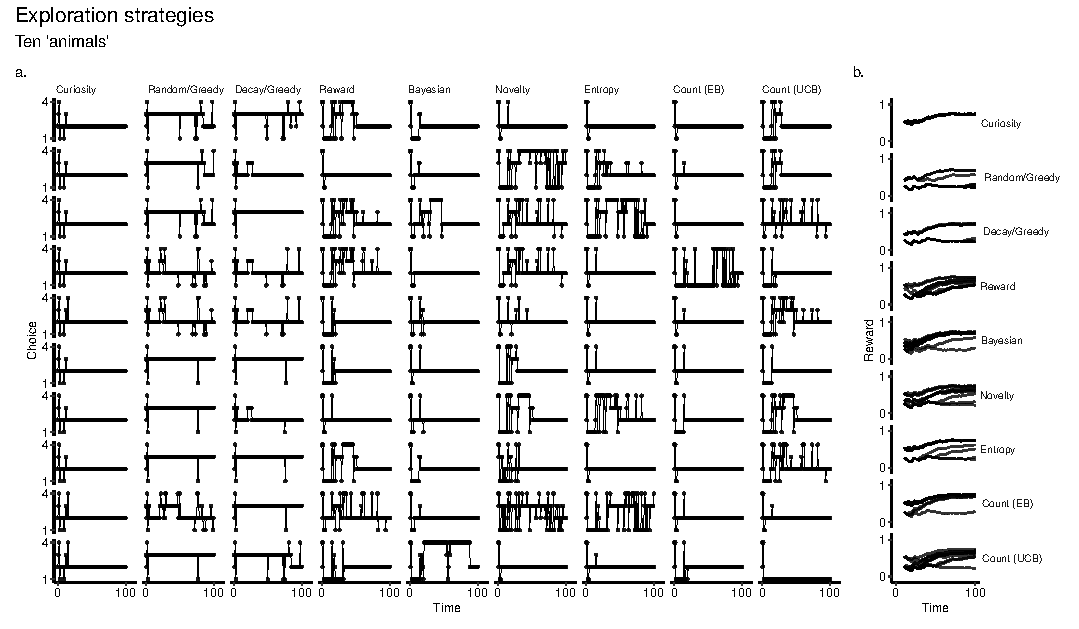
\includegraphics[width=1\linewidth]{dilemma-draft-elife/img/exploration1.pdf}}
	\end{fullwidth}
\end{figure}

\textit{Task 1.} is an information gathering task, which we discussed already above. \textit{Task 2} was designed to examine reward collection, in probabilistic reward setting very common in the decision making literature \citep{schonberg2007reinforcement,frank2004carrot,cavanagh2014conflict,jahfari2019cross,collins2014opponent,collins2017interactions,glascher2010states}. Rewards were 0 or 1. The best choice had a payout of $p(R=1) = 0.8$. This is a much higher average payout than the others ($p(R=1) = 0.2$). At no point does the task generate symbolic information. See, Fig.~\ref{fig:payout1}\textbf{b}. 

The results for Task 1 were discussed above. As for Task 2, we expected all the exploration strategies to succeed. While this was indeed the case, our deterministic curiosity was the top-performer in terms of median rewards collected, though by a small margin (Fig~\ref{fig:summary}\textbf{a}).

\textit{Task 3.} was designed with very sparse rewards \citep{Mniha,Silver2016b,Silver2018} and there were 10 choices, making this a more difficult task (Fig.~\ref{fig:payout1}\textbf{c}). Sparse rewards are a common problem in the natural world, where an animal may have to travel and search between each meal This is a difficult but not impossible task for vertebrates \citep{anderson1984optimal} and invertebrates \citep{westphal2006foraging}. That being said, most reinforcement learning algorithms will struggle in this setting because the thing they need to learn, that is rewards, are often absent. In this task we saw quite a bit more variation in performance, with the novelty-bonus strategy taking the top slot (this is the only time it does so).

\textit{Task 4.} was designed with deceptive rewards. By deceptive we mean that the best long-term option presents itself initially with a decreasing reward value (Fig.~\ref{fig:payout1}\textbf{d}). Such small deceptions abound in many natural contexts where one must often make short-term sacrifices \citep{internicola2012bumble}. It is well known that classic reinforcement learning will often struggle in this kind of task \citep{Lehman2011a,Sutton2018}. Here our deterministic curiosity is the only strategy that reaches above chance performance. Median performance of all other strategies are similar to the random control (Fig~\ref{fig:summary}\textbf{c}). 

\textit{Task 5} was designed to fool curiosity, our algorithm, by presenting information that was utterly irrelevant to reward collection, but had very high entropy and so ``interesting'' to our algorithm. We fully anticipated that this context would fool just our algorithm, with all other strategies performing well since they are largely agnostic to entropy. However, despite being designed to fail, deterministic curiosity still produced a competitive performance to the other strategies (Fig~\ref{fig:summary}\textbf{d}). 

\textit{Tasks 6-7} were designed as a pair, with both having 121 choices, and a complex payout structure. Tasks of this size are at the limit of human performance \citep{Wu2018}. We first trained all learners on \textit{Task 6}, then tested them in Task 7 which identical to 6, except the best payout arm is reset to be worst (Fig.~\ref{fig:payout1}\textbf{e}-\textbf{f}). In other words Tasks 6 and 7 were joined to measure learning in a high dimensional, but shifting, environments.

In Task 6 deterministic curiosity performed well, securing a second place finish. We note the Bayesian strategy  outperformed our approach. However, under the sudden non-stationarity in reward when switching tasks, the top Bayesian model became the worst on Task 7, and deterministic curiosity took the top spot. Compare Fig.~\ref{fig:summary}\textbf{e} to \textbf{f}. This is the robustness that we'd expect for any curiosity algorithm, whose main goal is to learn everything unbiased by other objectives. The environment and the objectives do change in real life, and so we must be prepared for this. Note how the other less-biased-toward-reward-value exploration models (count-based, novelty, and entropy models) also saw gains, to a lesser degree.

\subsection{Robustness}
A good choice of boredom $eta$ is critical for our definition of curiosity, and was optimized carefully. We show an example of this importance in Fig.~\ref{fig:boredom2}. On the left hand side we did a random search over 10000 possible parameters to find a value for $\eta$ that produced excellent results. (This was the same kind of search we did to achieve the results shown in Fig. ~\ref{fig:summary}. On the right hand side we choose a value for boredom we knew would lead to a poor relative result. We then ran the 100 different randomly generated simulations which gives us the results seen in Fig.~\ref{fig:boredom2}). 

Carefully optimized boredom converged far more quickly (Fig.~\ref{fig:boredom2}a-b), generating more reward over time (Fig.~\ref{fig:boredom2}c-d), and showed far more in consistency during exploration (Fig.~\ref{fig:boredom2}e-f). 

These experiments in setting $\eta$ are also useful in demonstrating the wide variance in behavior that is possible with a deterministic search. Exploration in these figures is deterministic, as prescribed by Eq.~\ref{eq:meta_greedy}. The environment was stochastic however and so the variations come from the environment changing what is learned, which then changes what the best learner should choose to learn next. 

\begin{figure}
	\begin{fullwidth}
	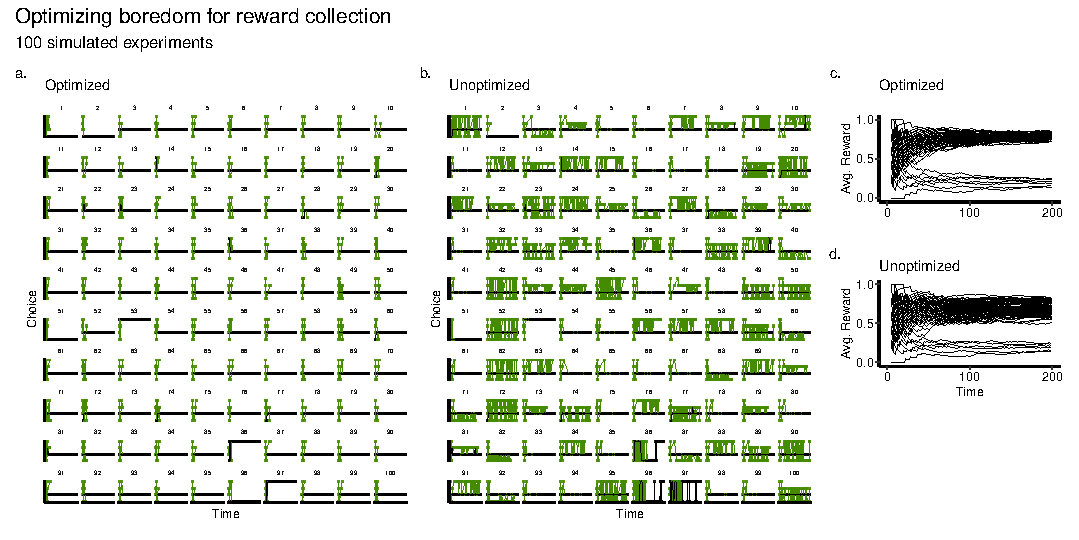
\includegraphics[width=.9\linewidth]{img/boredom2.pdf} 
	\caption{The importance of boredom during reward collection (Task 2). One hundred example experiments, each began with a different random seed. 
	\textbf{a}. Behavioral choices with optimized boredom.
	\textbf{b}. Behavioral choices with unoptimized boredom.
	\textbf{c,d}. Average reward as a function of time for optimized (c) and unoptimized (d) boredom.
	}
	\label{fig:boredom2} 
	\end{fullwidth}
\end{figure}

Unlike idealised simulations, animals cannot pre-optimize their search parameters for every task. We therefore explored reward collection as a function of 1000 randomly chosen model parameters, and reexamined performance on Tasks 1 and 7=6. These were chosen to represent an ``easy'' task, and a ``hard one''. These results are shown in Fig.~\ref{fig:robust}. 

As we observed in our other model comparisons, exploitation by deterministic curiosity produced top-3 performance on both tasks (Fig.~\ref{fig:robust}a-b). Most interesting is the performance for the worst parameters. Here deterministic curiosity was markedly better, with substantially less variability across different parameter schemes. We can explain this in the following way. All the other exploration strategies use parameters to tune the degree of exploration. With deterministic curiosity, however, we tune only when exploration should stop. The degree of exploration, the measure by how close it is to maximum entropy, is fixed by the model itself. It seems that here at least it is far more robust to tune the stopping point, rather than the degree of exploration.

\begin{figure}
	\begin{fullwidth}
	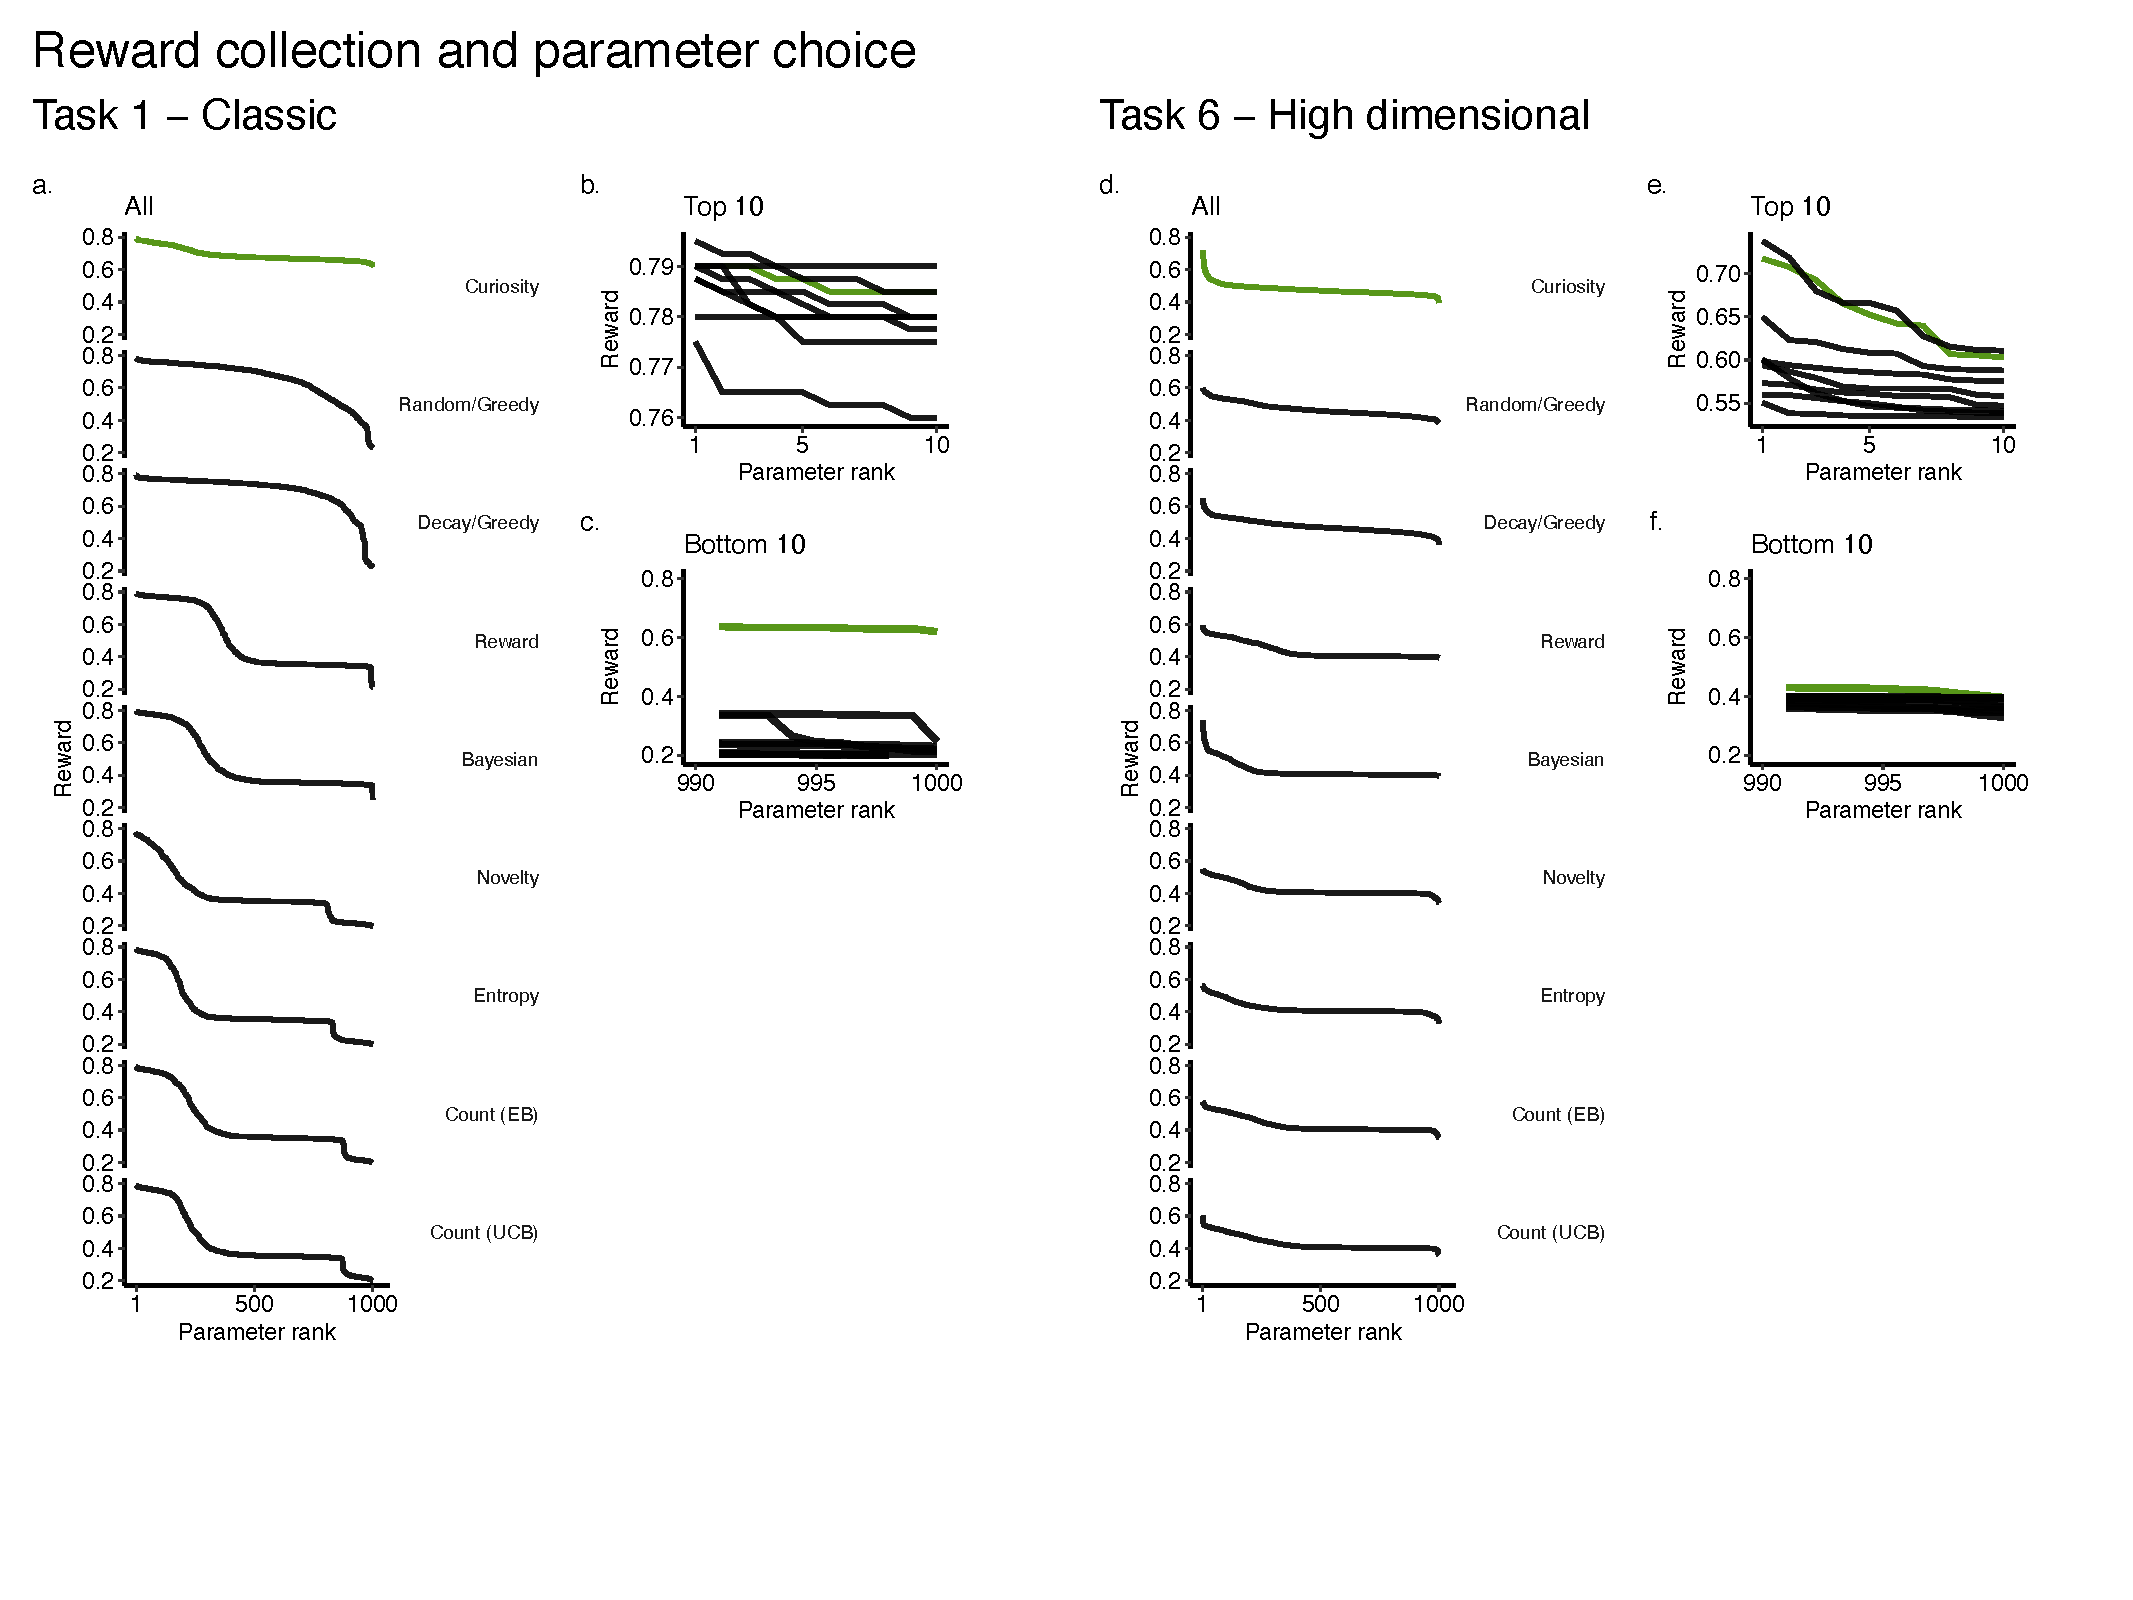
\includegraphics[width=0.8\linewidth]{img/robust.pdf} 
	\caption{Parameter selection and search performance (\textit{Task 2} and \textit{6}). We wanted to evaluate how robust performance was to poor and random hyperparameters. A very robustness exploration algorithm would produce strong performance with both the best parameter choices, and the worst parameter choices.   
	\textbf{a,d} Total reward for 1000 search hyperparameters, for each of strategies we considered.  
	\textbf{b,e} Performance with the top 10 hyperparameters, curiosity (green) compared to all the others.
	\textbf{c.f} Performance with the bottom 10 hyperparameters.
	}
	\figsupp{Adding noise to deterministic curiosity does degrade its performance. In this example control we added two levels of random noise. This only served to increase variability of convergence (a-c) and reduce the total rewards collected (d). Note: decision noise was modelled by sampling a Boltzmann distribution, as described in the \textit{Methods}.
    }{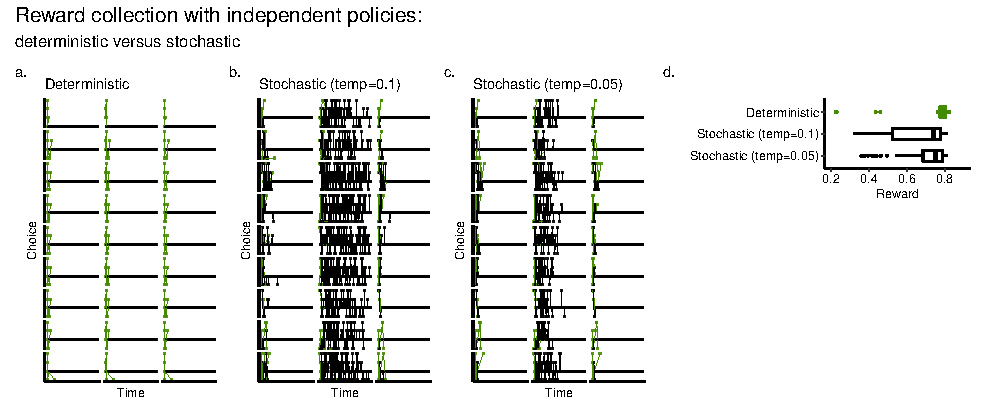
\includegraphics[width=1\linewidth]{img/independent2.pdf}}
    \figsupp{Noise across strategies. Adding noise to degrades performance to nearly the same degree (Task 2).
    }{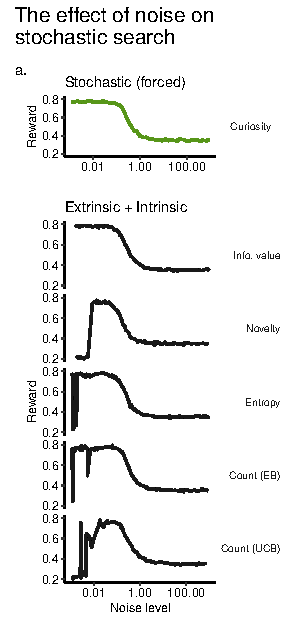
\includegraphics[width=0.3\linewidth]{dilemma-draft-elife/img/forced2.pdf}}
	\label{fig:robust}
	\end{fullwidth}
\end{figure}
